% Brindis en Rust --- Analisis y diseno OO del modulo de reservas
% Adaptación fiel del PDF original (Java/Spring) a Rust (Axum + sqlx).
% Cambios mínimos y justos para que sea idiomático en Rust, manteniendo
% trazabilidad con el documento base (mismos CU, RF, RN, figuras y tablas).
\documentclass[12pt]{article}
\usepackage[utf8]{inputenc}
\usepackage[T1]{fontenc}
% NOTA: es-noshorthands desactiva atajos babel (", <, >) que rompen TikZ (->)
% y listings con comillas dobles. No quitar.
\usepackage[spanish,es-noshorthands]{babel}
\usepackage{enumerate}
\usepackage{fancyhdr}
\usepackage[table]{xcolor}
\usepackage{float}
\usepackage{graphicx}
\usepackage{color}
\usepackage{caption}
\usepackage{mathtools}
\usepackage{amsmath}
\usepackage{tikz}
\usetikzlibrary{trees,positioning,arrows.meta,shapes.geometric,fit,calc}

% ---------- Estilo UML para las figuras (TikZ) ----------
\usetikzlibrary{shapes.multipart,arrows.meta,calc,positioning}
\definecolor{umlline}{HTML}{3A3A3A}
\definecolor{umliface}{HTML}{E4EDF7}
\definecolor{umlabs}{HTML}{FBF1D6}
\definecolor{umlutil}{HTML}{E6E6E6}
\definecolor{umlcls}{HTML}{F4F4F4}
\definecolor{umlnote}{HTML}{FFF8DC}
\definecolor{wfgris}{HTML}{8F8F8F}
\def\umlfs{\fontsize{7}{8.4}\selectfont}
\def\umlfst{\fontsize{5}{6}\selectfont}
\tikzset{
  umlbox/.style={rectangle split, rectangle split parts=3, draw=umlline, line width=0.5pt,
    font=\umlfs, align=left, inner xsep=4pt, inner ysep=2.2pt, anchor=north,
    rectangle split part align={center,left,left}, rectangle split empty part height=0pt},
  kc/.style={rectangle split part fill={umlcls,white,white}},
  ki/.style={rectangle split part fill={umliface,white,white}},
  ka/.style={rectangle split part fill={umlabs,white,white}},
  ku/.style={rectangle split part fill={umlutil,white,white}},
  gen/.style={umlline, line width=0.5pt, -{Triangle[open,length=7pt,width=7pt]}},
  real/.style={gen, dashed},
  dep/.style={umlline, line width=0.5pt, dashed, -{Straight Barb[length=5.5pt,width=7pt]}},
  asoc/.style={umlline, line width=0.5pt, -{Straight Barb[length=5.5pt,width=7pt]}},
  agg/.style={umlline, line width=0.5pt, {Diamond[open,length=9pt,width=6pt]}-{Straight Barb[length=5.5pt,width=7pt]}},
  el/.style={font=\umlfs\itshape, inner sep=1.2pt, text=umlline},
  mu/.style={font=\umlfs, inner sep=1pt, text=black},
  nota/.style={draw=umlline, fill=umlnote, line width=0.4pt, font=\umlfs, align=left,
    inner sep=4pt, anchor=north},
}
\def\umlst{}
\newcommand{\umlname}[2]{%
  \ifx\umlst\empty
    \if#1i{\umlfst\guillemotleft interface\guillemotright}\\[-1pt]\textbf{#2}%
    \else\if#1a\textbf{\textit{#2}}%
    \else\if#1u{\umlfst\guillemotleft utility\guillemotright}\\[-1pt]\textbf{#2}%
    \else\textbf{#2}\fi\fi\fi
  \else
    {\umlfst\guillemotleft\umlst\guillemotright}\\[-1pt]\if#1a\textbf{\textit{#2}}\else\textbf{#2}\fi%
  \fi}
% \umlcls{id}{top-center pos}{kind c|i|a|u}{width}{name}{attrs}{meths}
\newcommand{\umlcls}[7]{%
  \def\tA{#6}\def\tM{#7}%
  \ifx\tA\empty\ifx\tM\empty\def\np{1}\else\def\np{2}\fi\else\ifx\tM\empty\def\np{2}\else\def\np{3}\fi\fi
  \ifnum\np=1
    \node[umlbox,rectangle split parts=1,k#3,text width=#4] (#1) at (#2) {\umlname{#3}{#5}};
  \else\ifnum\np=2
    \node[umlbox,rectangle split parts=2,k#3,text width=#4] (#1) at (#2)
      {\umlname{#3}{#5}\nodepart{two}\ifx\tA\empty#7\else#6\fi};
  \else
    \node[umlbox,rectangle split parts=3,k#3,text width=#4] (#1) at (#2)
      {\umlname{#3}{#5}\nodepart{two}#6\nodepart{three}#7};
  \fi\fi
  \gdef\umlst{}}

\usepackage{amssymb}
\usepackage{xspace}
\usepackage[hidelinks]{hyperref}
\usepackage{booktabs}
\usepackage{tabularx}
\usepackage{listings}
\usepackage{url}
\usepackage{longtable}
\usepackage{array}
\usepackage{seqsplit}
\usepackage{microtype}
\setlength{\tabcolsep}{4pt}
\renewcommand{\arraystretch}{1.15}
\setlength{\emergencystretch}{3em}
\usepackage{lmodern}
\usepackage{textcomp}
\usepackage{upquote}

\hypersetup{
    colorlinks=false,
    pdfborder={0 0 0}
}

\setlength{\oddsidemargin}{0.5cm}
\setlength{\evensidemargin}{0.5cm}
\setlength{\topmargin}{-1.6cm}
\setlength{\leftmargin}{0.5cm}
\setlength{\rightmargin}{0.5cm}
\setlength{\textheight}{24.00cm}
\setlength{\textwidth}{15.00cm}
\parindent 0pt
\parskip 5pt

\pagestyle{fancy}
\renewcommand{\headrulewidth}{0pt}
\renewcommand{\footrulewidth}{0pt}
\setlength\headheight{35.0pt}
\addtolength{\textheight}{-35.0pt}

\IfFileExists{usa.png}{\rhead{\begin{picture}(0,0) \put(-56.7,0){
\includegraphics[width=30mm]{usa.png}} \end{picture}}}{}
\renewcommand{\headrulewidth}{0.5pt}

% ---------- Estilos de apoyo para los diagramas ----------
\tikzset{
  uc/.style={draw, ellipse, text width=3.6cm, minimum height=1.0cm,
             align=center, font=\scriptsize, inner sep=2pt},
  bloque/.style={draw, rounded corners, align=center, font=\scriptsize,
             minimum height=0.8cm, text width=2.6cm},
  hoja/.style={draw, rounded corners, align=left, font=\scriptsize,
             minimum height=0.6cm, text width=2.4cm, inner sep=3pt},
  wf/.style={draw, align=center, font=\scriptsize},
  wftxt/.style={font=\scriptsize, align=left, anchor=north west, inner sep=1pt},
  wfr/.style={draw=umlline, line width=0.55pt, rounded corners=2.5pt, fill=white},
  wfh/.style={draw=umlline, line width=0.45pt, fill=umlutil, rounded corners=1.5pt},
  wfb/.style={draw=wfgris!65, line width=0.35pt, rounded corners=1pt, fill=umlcls},
  wfd/.style={draw=umlline, line width=0.45pt, fill=umlline, rounded corners=1.5pt},
  wfo/.style={draw=umlline, line width=0.45pt, rounded corners=1.5pt, fill=white},
  wft/.style={font=\scriptsize\bfseries, text=umlline, inner sep=0pt},
  wfm/.style={font=\umlfst, text=umlline, inner sep=0.5pt},
  wfg/.style={font=\umlfst, text=wfgris, inner sep=0.5pt}
}

% Actor (monigote) reutilizable: {x}{y}{nombre-nodo}{etiqueta}
\newcommand{\actorNode}[4]{%
\begin{scope}[shift={(#1,#2)}]
  \draw[thick] (0,0.62) circle (0.15);
  \draw[thick] (0,0.47) -- (0,0.08);
  \draw[thick] (-0.24,0.35) -- (0.24,0.35);
  \draw[thick] (0,0.08) -- (-0.20,-0.25);
  \draw[thick] (0,0.08) -- (0.20,-0.25);
  \node[font=\scriptsize, align=center, anchor=north, text width=2.6cm] at (0,-0.34) {#4};
  \node[inner sep=0pt, minimum size=0pt] (#3) at (0,0.30) {};
\end{scope}}

\newcommand{\inc}{$\langle\langle$include$\rangle\rangle$}
\newcommand{\ext}{$\langle\langle$extend$\rangle\rangle$}

\lstdefinelanguage{Rust}{%
  morekeywords={trait,struct,enum,impl,pub,pub(crate),fn,mut,self,Self,mut,match,if,else,let,for,in,return,Ok,Err,Some,None,Box,dyn,async,await,where,use,mod,crate,as,ref},%
  sensitive=true,%
  morecomment=[l]{//},%
  morestring=[b]",%
}
\lstset{language=Rust,basicstyle=\ttfamily\small,breaklines=true,
  keywordstyle=\color{blue}\bfseries,commentstyle=\color{gray},
  stringstyle=\color{red!60!black},frame=single,numbers=left,numberstyle=\tiny,
  inputencoding=utf8,extendedchars=true,keepspaces=true,columns=fullflexible,
  literate={á}{{\'a}}1 {é}{{\'e}}1 {í}{{\'i}}1 {ó}{{\'o}}1 {ú}{{\'u}}1
           {Á}{{\'A}}1 {É}{{\'E}}1 {Í}{{\'I}}1 {Ó}{{\'O}}1 {Ú}{{\'U}}1
           {ñ}{{\~n}}1 {Ñ}{{\~N}}1 {¿}{{?`}}1 {¡}{{!`}}1
           {—}{{---}}1 {–}{{--}}1}

\begin{document}
\vspace{0.5cm}
\IfFileExists{usa.png}{\begin{figure}[H]
\centering

\includegraphics[scale = 0.4]{usa.png}
\end{figure}}{}
\vspace{1.5cm}

\begin{center}
\vskip 1cm
{\Large \bf Patrones de dise\~no de software}
\vskip 0.4cm
{\Large \bf An\'alisis y dise\~no orientado a objetos del m\'odulo de gesti\'on de reservas de restaurantes}
\vskip 0.3cm
{\large Brindis --- Sistema de reservas de restaurantes por ocasi\'on \textbf{(Implementaci\'on en Rust)}}
\vskip 0.8cm
{\bf Yslen Natalia Moreno Gutierrez \\ Jorge Antonio Garc\'ia Romero
\\
Karla Mariana Duque Callejas }
\vskip 3cm
{\it Universidad Sergio Arboleda \\ Escuela de ciencias exactas e ingenier\'ia \\
Bogot\'a D.C., 8 de octubre de 2026}
\end{center}

\clearpage

\tableofcontents
\newpage

\section{Introducción}
La reserva por ocasión (cumpleaños, aniversario, propuesta, romántica, negocios, casual) exige zona, decoración y servicio distintos. Brindis guía en 4 pasos (ocasión, mesas, pedido+extras, pago) con plano interactivo y bloqueo temporal de 5 min (RN03). Tres roles: cliente (general/VIP + strikes), empleado y administrador (hereda de empleado). Arquitectura MVC por capas + DAO (Alur et al., 2003) + 4 patrones (Gamma et al., 1994). \textbf{Cambio Rust:} Thymeleaf $\rightarrow$ Askama/Tera; Spring Controllers $\rightarrow$ handlers Axum; JDBC/ConexionBD $\rightarrow$ \texttt{sqlx} + \texttt{DbPool}; \texttt{BCrypt} $\rightarrow$ crate \texttt{bcrypt}; \texttt{PreparedStatement} $\rightarrow$ queries preparadas sqlx; transacciones sqlx (RNF02/RNF03).

\section{Planteamiento del problema}
Idéntico al original: asignación ineficiente y duplicados, pérdida de alergias/ocasión, venta extra no ofrecida, cancelaciones sin control, falta de control de acceso. Se requiere módulo que reserve sencillo y personalizado y que el personal controle mesas/horarios/reservas/pagos.

\section{Objetivos}
\subsection{Objetivo general}
Analizar, diseñar y desarrollar con el paradigma orientado a objetos (en Rust: traits + structs + enums) un módulo web de reservas con login y formulario para cliente y administrador, MVC por capas, 2 creacionales y 2 estructurales.
\subsection{Objetivos específicos}
\begin{enumerate}
\item Identificar actores, RF/RNF, RN y CU.
\item Diseñar modelo relacional y DAO.
\item Aplicar Factory Method y Builder en Rust.
\item Aplicar Proxy y Decorator en Rust.
\item Implementar UI intuitiva en 4 pasos con plano.
\end{enumerate}

\section{Alcance y propuesta de valor}
\subsection{Alcance}
Fase 1: login + formulario (cliente en línea, personal a nombre de cliente), consulta, cancelación con reembolso/strikes, agenda del día. Pagos simulados (se registra modalidad y comprobante, sin pasarela). Fase 2 diseñada: modificación, usuarios/mesas, estadísticas, reactivación, VIP automático. Fuera: pasarela real, app móvil.
\subsection{Propuesta de valor}
Ver Tabla~\ref{tab:valor}: ocasión $\rightarrow$ \texttt{enum Ocasion} + Builder; plano + bloqueo $\rightarrow$ servicio disponibilidad; pedido/extras $\rightarrow$ Decorator; VIP/strikes $\rightarrow$ Factory + Proxy; alertas $\rightarrow$ Decorator.
\begin{table}[h]\centering\caption{Elementos diferenciadores}\label{tab:valor}
\begin{tabular}{>{\raggedright\arraybackslash}p{3cm}>{\raggedright\arraybackslash}p{7cm}>{\raggedright\arraybackslash}p{3cm}}\toprule
Elemento & Descripción & Soporte\\\midrule
Reserva por ocasión & Elige qué celebra; sugiere zona y filtra decoración. & \texttt{Ocasion} y Builder\\
Plano + bloqueo & Zonas VIP/general/terraza; libre/reservada/bloqueada/seleccionada; bloqueo 5 min. & Disponibilidad\\
Pedido + extras & Preordena y contrata; total al instante. & Decorator\\
VIP y strikes & VIP flexible + pago en restaurante; tardías/inasistencias dan strikes. & Factory y Proxy\\
Restricciones & Alergias como alerta en agenda. & Decorator\\\bottomrule
\end{tabular}
\end{table}

\section{Análisis}
Enfoque Larman (2004); RF/RNF según Pressman y Maxim (2020).
\subsection{Actores y roles}
\begin{table}[H]\centering
\caption{Actores del sistema}\label{tab:actores}
{\small\textit{Actores del sistema}}\\[2pt]
\begin{tabular}{|>{\raggedright\arraybackslash}p{2.6cm}|>{\raggedright\arraybackslash}p{7.2cm}|>{\raggedright\arraybackslash}p{3.2cm}|}\hline
\textbf{Actor} & \textbf{Responsabilidades} & \textbf{{\textquestiondown}Qui{\'e}n lo crea?}\\\hline
Cliente (general o VIP) & Inicia sesi{\'o}n, registra reservas, elige mesas en el plano, agrega pedido y servicios extra, define el pago, consulta el estado de sus reservas y las modifica o cancela. & {\'E}l mismo desde la aplicaci{\'o}n, o un empleado.\\\hline
Empleado & Consulta la agenda del d{\'i}a, registra, modifica o cancela reservas a nombre de los clientes, crea clientes que no est{\'a}n registrados y actualiza el estado de las reservas. & Un administrador.\\\hline
Administrador & Hace todo lo que hace el empleado y, adem{\'a}s, consulta estad{\'i}sticas, crea empleados y administradores, asciende empleados a administrador, asciende clientes a VIP y activa o desactiva usuarios. & Otro administrador.\\\hline
\end{tabular}
\\[2pt]{\small\textit{Nota.} Elaboraci{\'o}n propia.}
\end{table}
\subsection{Requerimientos funcionales}
En la Tabla 3, la columna \textit{Fase} indica si el requerimiento se implementa en este parcial (1) o si queda dise{\~n}ado para una entrega posterior (2).
\begin{center}{\small\textbf{Tabla 3}}\\{\small\textit{Requerimientos funcionales}}\end{center}
\begin{longtable}{|p{1.2cm}|>{\raggedright\arraybackslash}p{8.2cm}|p{2.0cm}|c|}\hline
\textbf{ID} & \textbf{Descripci{\'o}n} & \textbf{Prioridad} & \textbf{Fase}\\\hline
\endhead
RF01 & Iniciar sesi{\'o}n con correo y contrase{\~n}a y redirigir al usuario a su panel seg{\'u}n su rol. & Alta & 1\\\hline
RF02 & Permitir que un cliente nuevo se registre por su cuenta; queda con rol cliente y tipo general. & Alta & 1\\\hline
RF03 & Restringir cada funci{\'o}n seg{\'u}n el rol del usuario autenticado y la propiedad de la reserva. & Alta & 1\\\hline
RF04 & Seleccionar la ocasi{\'o}n y el tipo de reserva (por mesas o restaurante completo). & Alta & 1\\\hline
RF05 & Consultar la disponibilidad por fecha, hora, n{\'u}mero de comensales y zona. & Alta & 1\\\hline
RF06 & Mostrar un plano interactivo y permitir seleccionar una o varias mesas, que quedan bloqueadas temporalmente. & Alta & 1\\\hline
RF07 & Agregar un pedido anticipado con productos de la carta. & Media & 1\\\hline
RF08 & Agregar servicios extra (decoraci{\'o}n y barra de c{\'o}cteles) y recalcular el valor total. & Alta & 1\\\hline
RF09 & Registrar restricciones alimentarias y observaciones. & Alta & 1\\\hline
RF10 & Seleccionar la modalidad de pago (adelanto, pago completo o pago en el restaurante cuando aplique) y emitir el comprobante. & Alta & 1\\\hline
RF11 & Confirmar la reserva, generar un c{\'o}digo {\'u}nico y mostrar el resumen. & Alta & 1\\\hline
RF12 & Permitir al personal registrar reservas a nombre de un cliente y crear al cliente si no existe. & Alta & 1\\\hline
RF13 & Permitir al cliente consultar sus reservas y el estado de cada una. & Media & 1\\\hline
RF14 & Cancelar una reserva aplicando la pol{\'i}tica de reembolso y de \textit{strikes}, y emitir el comprobante del reembolso. & Media & 1\\\hline
RF15 & Mostrar al personal la agenda del d{\'i}a con alertas, y permitirle cambiar el estado de las reservas. & Alta & 1\\\hline
RF16 & Modificar una reserva aplicando los precios vigentes y cobrando la diferencia del adelanto. & Media & 2\\\hline
RF17 & Enviar credenciales gen{\'e}ricas por correo a los clientes creados por el personal y exigir el cambio de contrase{\~n}a en el primer ingreso. & Media & 2\\\hline
RF18 & Permitir al administrador crear empleados y administradores, ascender usuarios y activarlos o desactivarlos. & Media & 2\\\hline
RF19 & Mostrar al administrador estad{\'i}sticas generales de reservas, ocupaci{\'o}n e ingresos. & Media & 2\\\hline
RF20 & Gestionar mesas, zonas, horarios de atenci{\'o}n, carta y planes de servicios extra. & Media & 2\\\hline
RF21 & Desactivar clientes por inactividad y permitir su reactivaci{\'o}n con un \textit{token} enviado por correo. & Baja & 2\\\hline
RF22 & Promover autom{\'a}ticamente a VIP a los clientes que cumplan los criterios definidos. & Baja & 2\\\hline
\end{longtable}
{\small\textit{Nota.} Elaboraci{\'o}n propia.}
\subsection{Requerimientos no funcionales}
\begin{center}{\small\textbf{Tabla 4}}\\{\small\textit{Requerimientos no funcionales}}\end{center}
\begin{longtable}{|p{1.4cm}|p{2.6cm}|>{\raggedright\arraybackslash}p{8.6cm}|}\hline
\textbf{ID} & \textbf{Atributo} & \textbf{Descripci{\'o}n}\\\hline
\endhead
RNF01 & Usabilidad & La reserva se completa en un m{\'a}ximo de cuatro pasos guiados y en menos de tres minutos para un usuario nuevo, siguiendo las heur{\'i}sticas de Nielsen (1993).\\\hline
RNF02 & Seguridad & Las contrase{\~n}as se almacenan con \textit{hash} BCrypt; cada operaci{\'o}n pasa por un control de acceso por rol; las consultas usan consultas preparadas para evitar inyecci{\'o}n SQL.\\\hline
RNF03 & Integridad & Una mesa no puede quedar en dos reservas activas con horarios cruzados; la verificaci{\'o}n, el registro de la reserva y su comprobante se ejecutan en una misma transacci{\'o}n.\\\hline
RNF04 & Rendimiento & Las consultas de disponibilidad responden en menos de dos segundos con hasta 50 mesas.\\\hline
RNF05 & Mantenibilidad & Agregar un nuevo rol, un nuevo tipo de servicio extra o una nueva ocasi{\'o}n no exige modificar las clases existentes (principio abierto/cerrado).\\\hline
RNF06 & Trazabilidad & Todo movimiento de dinero genera un comprobante con el empleado que lo proces{\'o}, si lo hubo.\\\hline
RNF07 & Portabilidad & La interfaz es adaptable (\textit{responsive}) y funciona en navegadores modernos de escritorio y m{\'o}vil.\\\hline
\end{longtable}
\subsection{Reglas de negocio}
Los valores num{\'e}ricos de la Tabla 5 (tiempos, porcentajes y umbrales) son par{\'a}metros configurables del sistema.
\begin{center}{\small\textbf{Tabla 5}}\\{\small\textit{Reglas de negocio}}\end{center}
\begin{longtable}{|p{1.2cm}|p{2.6cm}|>{\raggedright\arraybackslash}p{8.8cm}|}\hline
\textbf{ID} & \textbf{Tema} & \textbf{Regla}\\\hline
\endhead
RN01 & Duraci{\'o}n & Cada reserva dura 120 minutos por defecto. Una mesa no admite dos reservas activas (vigente o cliente en mesa) con franjas que se crucen.\\\hline
RN02 & Capacidad & La suma de las capacidades de las mesas seleccionadas debe ser igual o mayor que el n{\'u}mero de comensales.\\\hline
RN03 & Bloqueo temporal & Al seleccionar una mesa, esta queda bloqueada para esa franja durante cinco minutos. El bloqueo se libera al confirmar, al cancelar el proceso o al vencer el tiempo.\\\hline
RN04 & Restaurante completo & Una reserva de restaurante completo asocia autom{\'a}ticamente todas las mesas en servicio y exige que ninguna tenga reservas ni bloqueos en esa franja.\\\hline
RN05 & Horario & La reserva debe quedar dentro del horario de atenci{\'o}n y hacerse con al menos una hora de anticipaci{\'o}n y como m{\'a}ximo con 60 d{\'i}as.\\\hline
RN06 & Modalidad de pago & Adelanto: el cliente paga un porcentaje del total (30~\% por defecto). Completo: paga el 100~\%. En el restaurante: paga el 0~\% al reservar, y solo se permite si el cliente es VIP o si la reserva la registra el personal.\\\hline
RN07 & Precios y modificaciones & El precio de cada producto o servicio se guarda al agregarlo. Lo que se agrega en una modificaci{\'o}n usa el precio vigente en ese momento, no el de la reserva original. Si el total aumenta, el cliente paga la diferencia necesaria para mantener el porcentaje del adelanto. El saldo se liquida el d{\'i}a de la reserva.\\\hline
RN08 & Cancelaci{\'o}n de cliente general & Si cancela al menos cuatro horas antes, recibe el reembolso total de lo pagado. Si cancela despu{\'e}s, se retiene el 10~\% de lo pagado.\\\hline
RN09 & Cancelaci{\'o}n de cliente VIP & Puede cancelar sin penalidad hasta una hora antes. Si cancela despu{\'e}s, se retiene el 10~\% de lo pagado y recibe un \textit{strike}.\\\hline
RN10 & \textit{Strikes} & La inasistencia y el comportamiento indebido generan un \textit{strike}. Al tercer \textit{strike}, un cliente VIP pasa a ser general, y un cliente general no puede ser promovido a VIP.\\\hline
RN11 & Promoci{\'o}n a VIP & Un cliente pasa a VIP si lo asciende un administrador o, de forma autom{\'a}tica, si acumula 10 reservas completadas o un consumo de \$2.000.000 sin tener tres \textit{strikes}.\\\hline
RN12 & Creaci{\'o}n de usuarios & El cliente se registra solo o lo crea un empleado; el empleado solo lo crea un administrador; el administrador solo lo crea otro administrador. Un cliente creado por el personal recibe por correo una contrase{\~n}a gen{\'e}rica que debe cambiar en su primer ingreso.\\\hline
RN13 & Activaci{\'o}n & Un cliente sin actividad durante 180 d{\'i}as queda inactivo y puede reactivarse solo con un \textit{token} enviado a su correo. Un empleado o administrador desactivado solo puede ser reactivado por un administrador. Un administrador no puede desactivarse a s{\'i} mismo y siempre debe existir al menos un administrador activo.\\\hline
RN14 & Comprobantes & Cada movimiento de dinero (adelanto, liquidaci{\'o}n, reembolso total o parcial) genera un comprobante.\\\hline
RN15 & C{\'o}digo & Cada reserva tiene un c{\'o}digo alfanum{\'e}rico {\'u}nico de ocho caracteres.\\\hline
\end{longtable}
\subsection{Diagrama de casos de uso}
Administrador especializa a Empleado, por lo que hereda todos sus casos de uso. CU04 es el caso central: incluye siempre CU05 (seleccionar mesas) y CU06 (definir pago), y se extiende con CU07 (pedido anticipado) y CU08 (servicios extra).
\begin{figure}[H]\centering
{\small\textbf{Figura 1}}\\{\small\textit{Diagrama de casos de uso de Brindis}}\\[4pt]
\IfFileExists{../diagramas/brindis/Fig1_CasosUso.png}{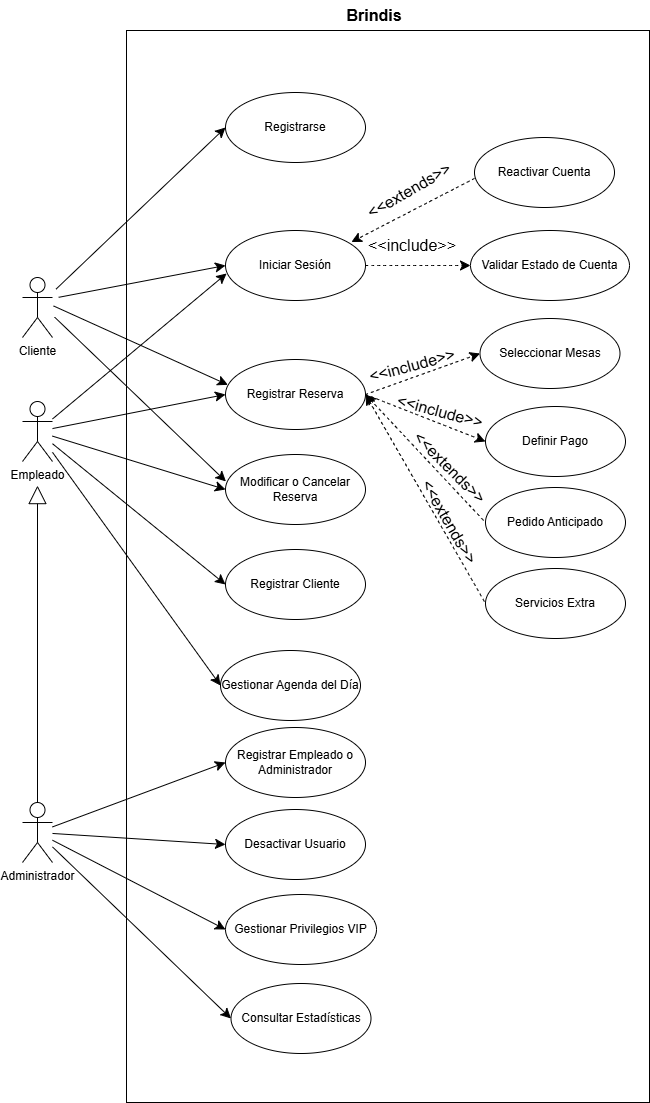
\includegraphics[width=0.95\linewidth]{../diagramas/brindis/Fig1_CasosUso.png}}{\fbox{\parbox{0.9\linewidth}{\small Para ver la figura, exportar \texttt{diagramas/brindis/Fig1\_CasosUso.drawio} a PNG (draw.io: Archivo \textgreater\ Exportar como \textgreater\ PNG, 300\,ppp) con el mismo nombre. Fuente guardada en el repo.}}}
\\[3pt]{\small\textit{Nota.} Elaboraci{\'o}n propia. La flecha con tri{\'a}ngulo vac{\'i}o entre actores indica que el administrador hereda los casos de uso del empleado. CU04 \textit{Registrar reserva} incluye CU05 y CU06 y se extiende con CU07 y CU08. \texttt{CU01} Iniciar sesi{\'o}n incluye \textit{Validar estado de cuenta} y se extiende con \textit{Registrarse} y \textit{Reactivar cuenta}.}
\end{figure}
An{\'a}lisis: el Cliente concentra el flujo de reserva (CU04) y sus extensiones opcionales de valor (pedido y extras), mientras que el personal comparte ese n{\'u}cleo y a{\~n}ade gesti{\'o}n (agenda CU10, modificar/cancelar CU09, registro de clientes CU11). El Administrador no repite casos: los hereda del Empleado y suma los propios (usuarios, VIP, estad{\'i}sticas). Los \textit{include} marcan lo obligatorio y los \textit{extend} lo opcional, por eso el total y los comprobantes solo aparecen cuando corresponde (RN07, RN14).
\subsection{Casos principales}
\begin{center}{\small\textbf{Tabla 6}}\\{\small\textit{Especificaci{\'o}n del caso de uso CU01 Iniciar sesi{\'o}n}}\end{center}
\begin{tabular}{|p{2.8cm}|>{\raggedright\arraybackslash}p{10.2cm}|}\hline
\textbf{Actores} & Cliente, empleado, administrador.\\\hline
\textbf{Precondici{\'o}n} & El usuario est{\'a} registrado y activo.\\\hline
\textbf{Flujo b{\'a}sico} & 1. El usuario ingresa su correo y contrase{\~n}a. 2. El sistema busca el usuario por correo y lo construye con la subclase de su rol. 3. El sistema compara la contrase{\~n}a con el \textit{hash} almacenado. 4. El sistema crea la sesi{\'o}n. 5. El sistema redirige al cliente a sus reservas y al personal a la agenda del d{\'i}a.\\\hline
\textbf{Flujos alternos} & 2a. El correo no existe o la contrase{\~n}a no coincide: se muestra ``Correo o contrase{\~n}a incorrectos'' sin indicar cu{\'a}l dato fall{\'o}. 2b. El usuario est{\'a} inactivo: se informa y, si es cliente, se ofrece enviar el \textit{token} de reactivaci{\'o}n. 4a. La contrase{\~n}a es gen{\'e}rica: se exige cambiarla antes de continuar.\\\hline
\textbf{Postcondici{\'o}n} & Existe una sesi{\'o}n activa asociada al usuario y a su rol.\\\hline
\end{tabular}

\begin{center}{\small\textbf{Tabla 7}}\\{\small\textit{Especificaci{\'o}n del caso de uso CU04 Registrar reserva}}\end{center}
\begin{longtable}{|p{2.8cm}|>{\raggedright\arraybackslash}p{10.2cm}|}\hline
\textbf{Actores} & Cliente (reserva en l{\'i}nea), empleado y administrador (reserva a nombre de un cliente).\\\hline
\textbf{Precondici{\'o}n} & El usuario inici{\'o} sesi{\'o}n.\\\hline
\textbf{Flujo b{\'a}sico} & 1. El usuario elige la ocasi{\'o}n, el tipo de reserva, la fecha, la hora y el n{\'u}mero de comensales. 2. El sistema muestra el plano con el estado de cada mesa en esa franja y resalta la zona sugerida para la ocasi{\'o}n. 3. El usuario selecciona una o varias mesas (CU05) y el sistema las bloquea cinco minutos. 4. El usuario agrega, si lo desea, un pedido anticipado (CU07) y servicios extra (CU08), e indica restricciones alimentarias. 5. El sistema recalcula el total. 6. El usuario define la modalidad y el medio de pago (CU06). 7. El usuario confirma. 8. El sistema verifica los permisos, valida las reglas RN01 a RN06, guarda la reserva, emite el comprobante y muestra el c{\'o}digo.\\\hline
\textbf{Flujos alternos} & 1a. Si el actor es del personal, primero busca al cliente por documento; si no existe, lo registra (CU11). 1b. Si elige restaurante completo, el sistema omite el paso 3 y asocia todas las mesas (RN04). 3a. La capacidad seleccionada no alcanza: el sistema lo indica y no permite continuar. 8a. El bloqueo venci{\'o} y otro usuario tom{\'o} la mesa: el sistema informa y regresa al paso 2. 8b. Se eligi{\'o} pago en el restaurante sin cumplir RN06: el sistema lo rechaza.\\\hline
\textbf{Postcondici{\'o}n} & La reserva queda en estado \textit{vigente}, con su c{\'o}digo, sus mesas, su detalle de pago y su comprobante.\\\hline
\end{longtable}
{\small\textit{Nota.} Elaboraci{\'o}n propia.}

\begin{center}{\small\textbf{Tabla 8}}\\{\small\textit{Especificaci{\'o}n del caso de uso CU09 Modificar o cancelar reserva (cancelaci{\'o}n)}}\end{center}
\begin{tabular}{|p{2.8cm}|>{\raggedright\arraybackslash}p{10.2cm}|}\hline
\textbf{Actores} & Cliente (sus propias reservas), empleado y administrador.\\\hline
\textbf{Precondici{\'o}n} & La reserva est{\'a} vigente.\\\hline
\textbf{Flujo b{\'a}sico} & 1. El usuario elige la reserva y la opci{\'o}n cancelar. 2. El sistema calcula las horas que faltan y, seg{\'u}n el tipo de cliente, el valor a reembolsar (RN08, RN09). 3. El sistema muestra el reembolso y la retenci{\'o}n. 4. El usuario confirma. 5. El sistema cambia el estado a \textit{cancelada}, libera las mesas, emite el comprobante de reembolso total o parcial y, si aplica, registra un \textit{strike}.\\\hline
\textbf{Flujos alternos} & 1a. Un cliente intenta cancelar una reserva ajena: el control de acceso lo rechaza. 2a. No hubo pagos: la reserva se cancela sin comprobante.\\\hline
\textbf{Postcondici{\'o}n} & La reserva queda cancelada y el reembolso queda registrado.\\\hline
\end{tabular}
{\small\textit{Nota.} Elaboraci{\'o}n propia.}

\begin{center}{\small\textbf{Tabla 9}}\\{\small\textit{Especificaci{\'o}n del caso de uso CU10 Gestionar agenda del d{\'i}a}}\end{center}
\begin{tabular}{|p{2.8cm}|>{\raggedright\arraybackslash}p{10.2cm}|}\hline
\textbf{Actores} & Empleado, administrador.\\\hline
\textbf{Precondici{\'o}n} & El usuario inici{\'o} sesi{\'o}n con un rol del personal.\\\hline
\textbf{Flujo b{\'a}sico} & 1. El usuario abre la agenda. 2. El sistema muestra las reservas del d{\'i}a ordenadas por hora, con el cliente (y si es VIP), las mesas, la ocasi{\'o}n, las alertas de restricciones y las indicaciones de servicio. 3. El usuario cambia el estado de una reserva: \textit{cliente en mesa} al llegar, \textit{completada} al liquidar el saldo o \textit{inasistida}. 4. El sistema guarda el cambio; si es una inasistencia, registra un \textit{strike}; si es una liquidaci{\'o}n, emite el comprobante.\\\hline
\textbf{Flujos alternos} & 1a. El usuario elige otra fecha. 3a. La transici{\'o}n no es v{\'a}lida (por ejemplo, completar una reserva cancelada): el sistema la rechaza.\\\hline
\textbf{Postcondici{\'o}n} & El estado de la reserva queda actualizado.\\\hline
\end{tabular}
{\small\textit{Nota.} Elaboraci{\'o}n propia.}
\subsection{Ciclo de vida}
VIGENTE $\rightarrow$ CLIENTE\_EN\_MESA $\rightarrow$ COMPLETADA; VIGENTE $\rightarrow$ CANCELADA/INASISTIDA; la modificaci{\'o}n se hace sobre una reserva vigente. La Figura 2 resume los estados de una reserva y los eventos que producen cada transici{\'o}n.
\begin{figure}[H]\centering
{\small\textbf{Figura 2}}\\{\small\textit{Diagrama de estados de la reserva}}\\[4pt]
\begin{tikzpicture}[
  estado/.style={draw, rounded corners=2pt, font=\scriptsize, minimum height=0.85cm, minimum width=2.2cm, align=center, fill=umlcls},
  ev/.style={font=\scriptsize, inner sep=1.5pt, text=umlline},
  fl/.style={umlline, line width=0.5pt, -{Straight Barb[length=5.5pt,width=7pt]}},
]
  % --- inicio y fin ---
  \node[circle, fill=black, minimum size=0.28cm, inner sep=0pt] (ini) at (-1.6,0) {};
  \node[circle, draw=umlline, fill=white, double, double distance=1.3pt, minimum size=0.34cm, inner sep=0pt] (fin) at (12.2,2.2) {};
  \node[font=\scriptsize, anchor=south] at (ini.north) {Inicio};
  \node[font=\scriptsize, anchor=south] at (fin.north) {Fin};
  % --- estados ---
  \node[estado] (vig) at (2.4,0) {VIGENTE};
  \node[estado] (can) at (2.4,2.2) {CANCELADA};
  \node[estado] (ina) at (7.4,0) {INASISTIDA};
  \node[estado] (cli) at (8.0,-2.4) {CLIENTE\_EN\_MESA};
  \node[estado] (com) at (12.2,-2.4) {COMPLETADA};
  % --- crear reserva ---
  \draw[fl] (ini) -- (vig.west);
  \node[ev, anchor=south] at ($(ini.east)!.5!(vig.west)+(0,0.04)$) {crear reserva};
  % --- cancelar (sube) ---
  \draw[fl] (vig.north) -- (can.south);
  \node[ev, anchor=west, align=left, text width=2.8cm] at ($(vig.north)!.5!(can.south)+(0.12,0)$) {cliente o personal cancelan la reserva};
  % --- cancelada -> fin ---
  \draw[fl] (can.east) -- (fin.west);
  % --- no asiste ---
  \draw[fl] (vig.east) -- (ina.west);
  \node[ev, anchor=south] at ($(vig.east)!.5!(ina.west)+(0,0.12)$) {comensal no asiste};
  % --- inasistida -> fin ---
  \draw[fl] (ina.north east) -- (fin.south);
  % --- asiste ---
  \coordinate (ds) at ($(vig.south)+(0.9,0)$);
  \draw[fl] (ds) -- (cli.west);
  \node[ev, rotate=-30, anchor=south, font=\umlfst] at ($(ds)!.5!(cli.west)+(0,0.14)$) {comensal asiste a la hora pactada};
  % --- liquidar ---
  \draw[fl] (cli.east) -- (com.west);
  \node[ev, anchor=south] at ($(cli.east)!.5!(com.west)+(0,0.06)$) {liquidar cuenta};
  % --- completada -> fin ---
  \draw[fl] (com.north) -- (fin.south);
  % --- autotransicion: modificar ---
  \draw[fl] ($(vig.south)+(-0.75,0)$) .. controls +(-0.25,-1.2) and +(0.6,-1.2) .. ($(vig.south)+(-0.15,0)$);
  \node[ev, anchor=north, align=center] at ($(vig.south)+(-0.45,-1.5)$) {cliente o personal\\modifican la reserva};
\end{tikzpicture}
\\[3pt]{\small\textit{Nota.} Elaboraci{\'o}n propia. Las transiciones inv{\'a}lidas (por ejemplo, completar una reserva cancelada) se rechazan en \texttt{cambiar\_estado()} (\texttt{src/dominio.rs}).}
\end{figure}

\section{Diseño}
\subsection{Arquitectura MVC por capas}
La Vista presenta la informaci\'on, el Controlador atiende las peticiones y el Modelo contiene la l\'ogica y los datos. Para separar mejor las responsabilidades, el modelo se divide a su vez en tres capas internas: servicios y patrones, acceso a datos y entidades; la Figura 3 muestra la organizaci{\'o}n resultante. Lo cr\'itico: los controladores no acceden a la l\'ogica de reservas sin pasar por el control de acceso (proxies de servicio); la verificaci\'on de cruces, el registro de la reserva y su comprobante se ejecutan en una misma transacci\'on.
\begin{figure}[H]\centering
{\small\textbf{Figura 3}}\\{\small\textit{Arquitectura MVC por capas}}\\[4pt]
\begin{tikzpicture}[
  band/.style={draw=umlline, line width=0.5pt, rounded corners=3pt, fill=white},
  chip/.style={draw=umlline, line width=0.4pt, fill=umlutil, rounded corners=1.5pt, font=\umlfst, inner sep=2.6pt, minimum height=0.42cm, align=center},
  tit/.style={font=\scriptsize\bfseries, text=umlline, align=center, inner sep=0pt},
  lb/.style={font=\umlfst, text=umlline, inner sep=1.5pt},
  fl/.style={umlline, line width=0.5pt, -{Straight Barb[length=5.5pt,width=7pt]}},
  flb/.style={umlline, line width=0.5pt, {Straight Barb[length=5.5pt,width=7pt]}-{Straight Barb[length=5.5pt,width=7pt]}},
]
  % --- Vista ---
  \node[band, minimum width=10.6cm, minimum height=1.35cm, anchor=north west] (vista) at (0,0) {};
  \node[tit, anchor=west] at ($(vista.west)+(0.25,0)$) {Vista};
  \node[chip] at (3.05,-0.44) {plantillas Askama};
  \node[chip] at (6.15,-0.44) {plano.js y ui.js};
  \node[chip] at (9.15,-0.44) {tema.css y fuentes};
  \node[chip] at (5.75,-0.98) {HTML + CSS + JS vanilla (sin librer{\'i}as)};
  % --- Controlador ---
  \node[band, minimum width=10.6cm, minimum height=0.95cm, anchor=north west] (ctrl) at (0,-2.2) {};
  \node[tit, anchor=west] at ($(ctrl.west)+(0.25,0)$) {Controlador\\(Axum)};
  \node[chip] at (3.15,-2.67) {AuthController};
  \node[chip] at (6.05,-2.67) {ReservaController};
  \node[chip] at (8.95,-2.67) {PersonalController};
  % --- Modelo: servicios y patrones ---
  \node[band, minimum width=10.6cm, minimum height=2.35cm, anchor=north west] (serv) at (0,-4.0) {};
  \node[tit, anchor=west, text width=1.7cm] at ($(serv.west)+(0.25,0)$) {Modelo:\\servicios y patrones};
  \node[chip] at (3.1,-4.5) {UsuarioServiceProxy};
  \node[chip] at (6.2,-4.5) {ReservaServiceProxy};
  \node[chip] at (9.15,-4.5) {UsuarioServiceImpl};
  \node[chip] at (3.1,-5.08) {ReservaServiceImpl};
  \node[chip] at (6.2,-5.08) {UsuarioFactory};
  \node[chip] at (9.15,-5.08) {ReservaBuilder};
  \node[chip] at (3.35,-5.66) {ComponenteReserva\\(decoradores)};
  \node[chip] at (6.35,-5.66) {DisponibilidadService};
  \node[chip] at (9.15,-5.66) {PagoService};
  % --- Modelo: acceso a datos ---
  \node[band, minimum width=10.6cm, minimum height=0.95cm, anchor=north west] (dao) at (0,-6.9) {};
  \node[tit, anchor=west] at ($(dao.west)+(0.25,0)$) {Modelo:\\acceso a datos};
  \node[chip] at (3.3,-7.37) {traits *Dao};
  \node[chip] at (6.2,-7.37) {impls *Sqlx};
  \node[chip] at (8.85,-7.37) {DbPool};
  % --- Base de datos ---
  \node[band, minimum width=10.6cm, minimum height=0.7cm, anchor=north west] (bd) at (0,-8.4) {};
  \node[tit, anchor=west] at ($(bd.west)+(0.25,0)$) {Base de\\datos};
  \node[chip] at (4.1,-8.75) {brindis\_db};
  \node[lb, anchor=west] at (5.65,-8.75) {(13 tablas, 3FN)};
  % --- Modelo: entidades (lateral) ---
  \node[band, minimum width=3.2cm, minimum height=3.85cm, anchor=north west] (ent) at (11.2,-4.0) {};
  \node[tit] at (12.8,-4.45) {Modelo:\\entidades};
  \node[lb, align=center] at (12.8,-5.75) {structs del dominio\\y DTO\\(Usuario, Reserva, Mesa,\\Plan...)};
  % --- dependencias hacia las entidades ---
  \coordinate (e1) at (ent.west |- serv.east);
  \coordinate (e2) at (ent.west |- dao.east);
  \draw[fl, dashed] (serv.east) -- (e1);
  \node[lb, anchor=south] at ($(serv.east)!.5!(e1)+(0,0.03)$) {usan};
  \draw[fl, dashed] (dao.east) -- (e2);
  \node[lb, anchor=south] at ($(dao.east)!.5!(e2)+(0,0.03)$) {usan};
  % --- flujo vertical ---
  \draw[flb] (vista.south) -- (ctrl.north);
  \node[lb, anchor=west] at ($(vista.south)!.5!(ctrl.north)+(0.1,0.02)$) {peticiones y respuestas};
  \draw[fl] (ctrl.south) -- (serv.north);
  \node[lb, anchor=west] at ($(ctrl.south)!.5!(serv.north)+(0.1,0)$) {usa las interfaces de servicio};
  \draw[fl] (serv.south) -- (dao.north);
  \node[lb, anchor=west] at ($(serv.south)!.5!(dao.north)+(0.1,0)$) {consultas};
  \draw[flb] (dao.south) -- (bd.north);
  \node[lb, anchor=west] at ($(dao.south)!.5!(bd.north)+(0.1,0)$) {SQL (pool)};
\end{tikzpicture}
\\[3pt]{\small\textit{Nota.} Elaboraci{\'o}n propia. Las flechas punteadas indican dependencia de uso: los servicios y los DAO usan las entidades del dominio; la vista no conoce al modelo y el controlador solo conoce las interfaces de servicio (proxies).}
\end{figure}
\subsection{Diagrama de clases del modelo}
Usuario es abstracta y se especializa en Cliente y Empleado; Administrador hereda de Empleado, lo que expresa que puede hacer todo lo del personal. Lo cr\'itico: la Reserva pertenece a un Cliente, puede haber sido creada por un Empleado, ocupa una o varias Mesas y se compone de su pedido anticipado y sus servicios extra. La enumeraci\'on Ocasion sostiene la reserva por ocasi\'on: cada valor conoce la zona sugerida y la decoraci\'on ofrecida.
\begin{figure}[H]\centering
{\small\textbf{Figura 4}}\\{\small\textit{Diagrama de clases del modelo (entidades)}}\\[4pt]
\IfFileExists{../diagramas/brindis/Fig4_DiagramaClases.png}{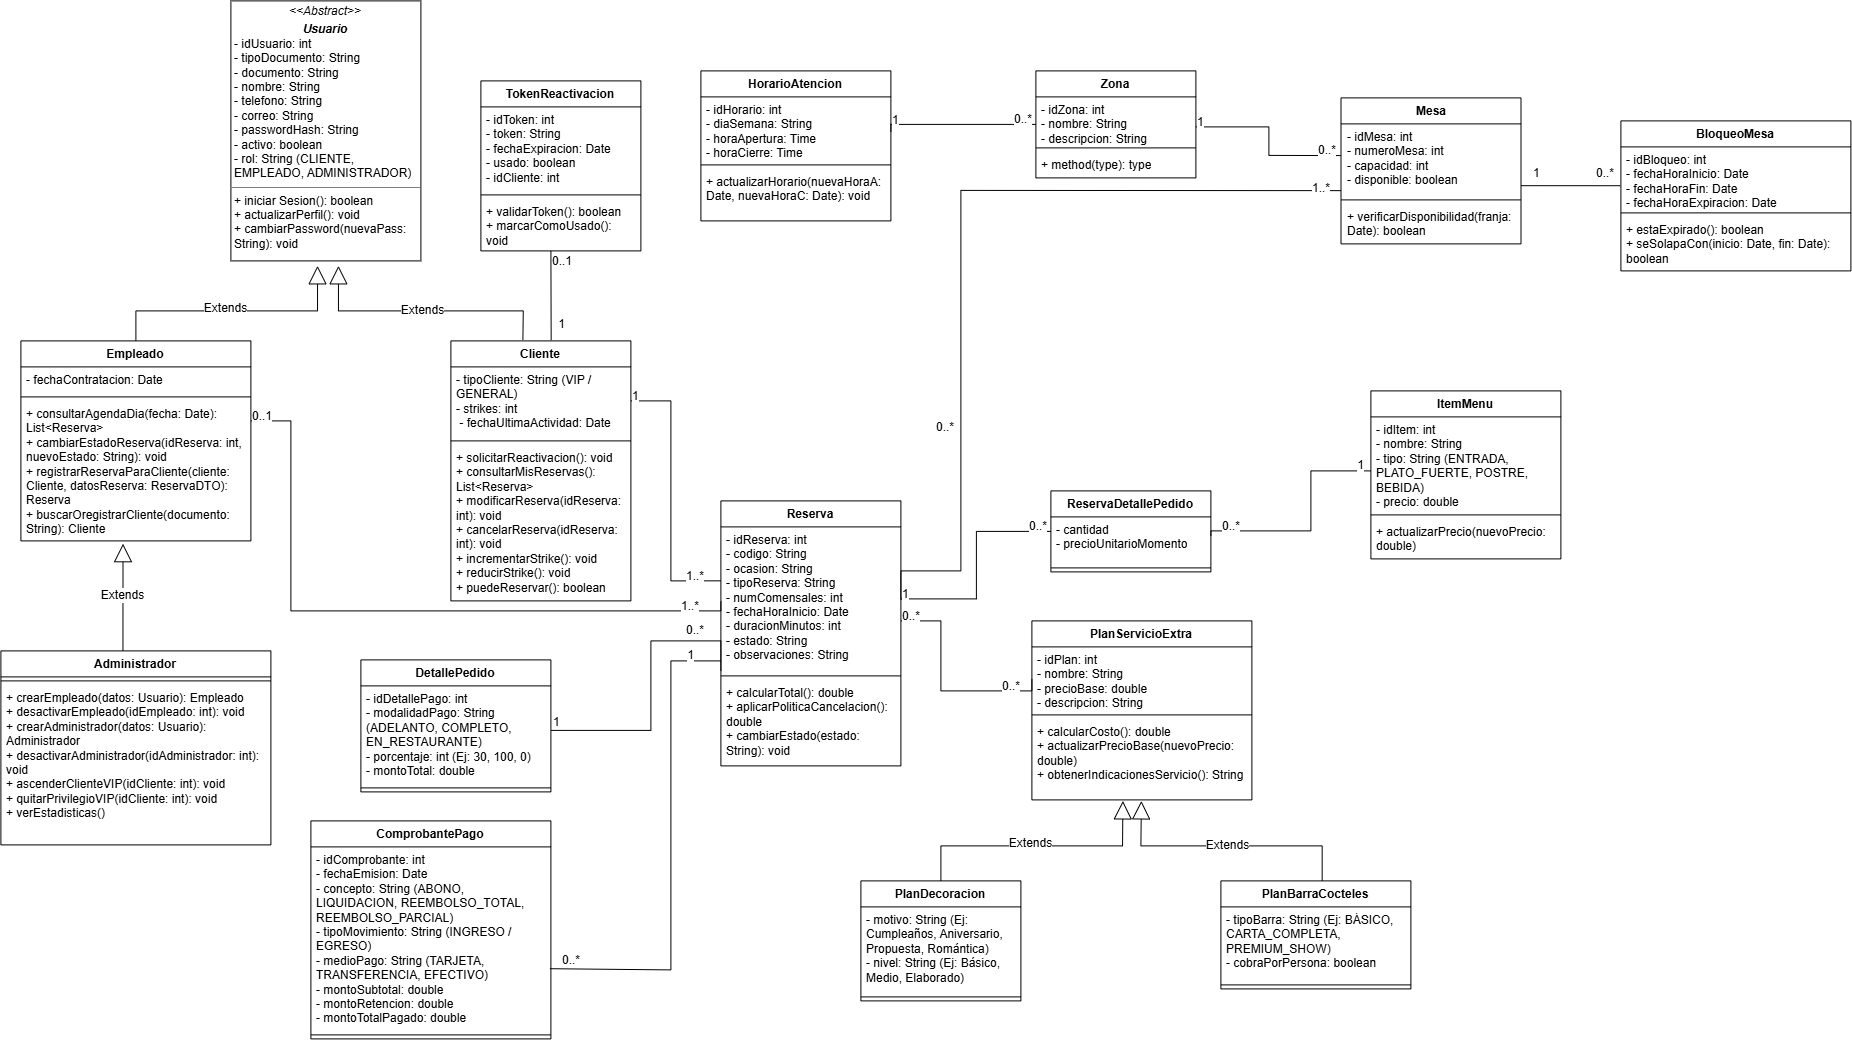
\includegraphics[width=0.95\linewidth]{../diagramas/brindis/Fig4_DiagramaClases.png}}{\fbox{\parbox{0.9\linewidth}{\small Para ver la figura, exportar \texttt{diagramas/brindis/Fig4\_DiagramaClases.drawio} a PNG (draw.io: Archivo \textgreater\ Exportar como \textgreater\ PNG, 300\,ppp) con el mismo nombre. Fuente guardada en el repo.}}}
\\[3pt]{\small\textit{Nota.} Elaboraci{\'o}n propia. Se omiten los m{\'e}todos \textit{get} y \textit{set}. El rombo relleno indica composici{\'o}n. Las relaciones de muchos a muchos (por ejemplo, Reserva con Mesa, ItemMenu o PlanServicioExtra) se solucionan en la base de datos con una tabla intermedia (reserva\_mesa, reserva\_detalle\_pedido, reserva\_servicio\_extra, que adem{\'a}s conservan el precio vigente RN07), pero por facilidad de lectura el diagrama las muestra como asociaci{\'o}n directa con su multiplicidad; impl{\'i}citamente la l{\'o}gica ha de contemplar esas tablas intermedias.}
\end{figure}
An{\'a}lisis: la jerarqu{\'i}a de usuarios concentra en \textit{Usuario} lo com{\'u}n (identidad, credenciales, estado) y deja en cada subclase lo propio (strikes y VIP en Cliente, legajo y agenda en Empleado, gesti{\'o}n en Administrador), lo que sostiene a \textit{Factory Method} y al \textit{Proxy}. La Reserva es el agregado central: sus composiciones (detalle de pedido y de pago, comprobantes) mueren con ella, mientras que Mesa, Zona, Horario y Planes existen por s{\'i} mismos y solo se asocian con su multiplicidad (\texttt{1}, \texttt{0..1}, \texttt{1..*}, \texttt{0..*}). BloqueoMesa y TokenReactivacion modelan lo temporal (RN03, RN13) sin contaminar a Mesa ni a Cliente.
\begin{center}{\small\textbf{Tabla 10}}\\{\small\textit{Valores de la enumeraci{\'o}n Ocasion}}\end{center}
{\footnotesize
\begin{tabular}{|>{\raggedright\arraybackslash}p{2.6cm}|>{\raggedright\arraybackslash}p{2.4cm}|>{\raggedright\arraybackslash}p{2.8cm}|>{\raggedright\arraybackslash}p{5.0cm}|}\hline
\textbf{Ocasi{\'o}n} & \textbf{Zona sugerida} & \textbf{Decoraci{\'o}n ofrecida} & \textbf{Indicaci{\'o}n para el personal}\\\hline
CUMPLEANOS & General & Cumplea{\~n}os & Preparar la canci{\'o}n al servir el postre.\\\hline
ANIVERSARIO & VIP & Aniversario & Luz tenue y m{\'u}sica suave.\\\hline
PROPUESTA & VIP & Propuesta & Coordinar con el cliente el momento de la propuesta.\\\hline
ROMANTICA & Terraza & Rom{\'a}ntica & Mesa apartada y servicio discreto.\\\hline
NEGOCIOS & VIP & Ninguna & Servicio {\'a}gil y sin interrupciones.\\\hline
CASUAL & Cualquiera & Ninguna & Servicio est{\'a}ndar.\\\hline
\end{tabular}
}
\subsection{Modelo relacional \texttt{brindis\_db}}
13 tablas normalizadas 3FN (Elmasri y Navathe, 2016): usuario, token\_reactivacion, mesa (solo DISPONIBLE/FUERA\_DE\_SERVICIO; reservada/bloqueada se calcula por franja desde reserva\_mesa + bloqueo\_mesa), horario\_atencion, reserva (codigo único, id\_creador nulable), reserva\_mesa, item\_menu, reserva\_detalle\_pedido (precio congelado), plan\_servicio\_extra, reserva\_servicio\_extra (precio congelado), detalle\_pago (0--100), comprobante\_pago (id\_empleado nulable). Índices en reserva\_mesa.id\_mesa y reserva.fecha\_hora\_inicio (RN01). Script SQL en Anexo.
\subsection{Diagrama de clases DAO}
\begin{figure}[H]\centering
{\small\textbf{Figura 6}}\\{\small\textit{Diagrama de clases DAO}}\\[4pt]
\begin{tikzpicture}
\umlcls{gen}{3.2,0}{i}{6.0cm}{GenericDAO<T, Id>}{}{+obtener()\ \ +listar()\ \ +guardar()\ \ +eliminar()}
\coordinate (trk) at ($(gen.south west)+(0.45,0)$);
% --- Interfaces DAO ---
\umlcls{u}{$(gen.south)+(0.1,-1.1)$}{i}{4.3cm}{UsuarioDAO}{}{+buscar\_por\_correo() : Usuario}
\umlcls{m}{$(u.south)+(0,-0.4)$}{i}{4.3cm}{MesaDAO}{}{+en\_servicio() : Lista}
\umlcls{r}{$(m.south)+(0,-0.4)$}{i}{4.3cm}{ReservaDAO}{}{+hay\_cruce() : boolean}
\umlcls{c}{$(r.south)+(0,-0.4)$}{i}{4.3cm}{CatalogoDAO}{}{}
\umlcls{p}{$(c.south)+(0,-0.4)$}{i}{4.3cm}{PagoDAO}{}{+emitir\_comprobante() : id}
% --- Implementaciones ---
\umlcls{ui}{$(u.north)+(5.5,-0.25)$}{c}{3.0cm}{UsuarioDAOImpl}{}{}
\umlcls{mi}{$(m.north)+(5.5,-0.25)$}{c}{3.0cm}{MesaDAOImpl}{}{}
\umlcls{ri}{$(r.north)+(5.5,-0.25)$}{c}{3.0cm}{ReservaDAOImpl}{}{}
\umlcls{ci}{$(c.north)+(5.5,-0.12)$}{c}{3.0cm}{CatalogoDAOImpl}{}{}
\umlcls{pi}{$(p.north)+(5.5,-0.25)$}{c}{3.0cm}{PagoDAOImpl}{}{}
% --- Conexion ---
\umlcls{pool}{$(ri.north)+(3.9,0.1)$}{u}{2.3cm}{ConexionBD}{-url : String}{}
% --- Generalizacion: interfaces -> GenericDAO (tronco a la izquierda) ---
\foreach \x in {u,m,r,c,p}{ \draw[gen] (\x.west) -- (\x.west -| trk) -- (trk); }
% --- Realizacion: impl -> interfaz ---
\foreach \i/\x in {ui/u,mi/m,ri/r,ci/c,pi/p}{ \draw[real] (\i.west) -- (\i.west -| \x.east); }
% --- Asociacion con multiplicidad: muchos DAOImpl comparten una ConexionBD ---
\coordinate (bus) at ($(pool.west)+(-0.95,0)$);
\foreach \i in {ui,mi,ri,ci,pi}{
  \draw[umlline,line width=0.5pt] (\i.east) -- (\i.east -| bus);
  \node[mu] at ($(\i.east)+(0.22,0.16)$) {*};
}
\draw[umlline,line width=0.5pt] (ui.east -| bus) -- (pi.east -| bus);
\draw[asoc] (bus |- pool.west) -- (pool.west);
\node[mu] at ($(pool.west)+(-0.3,0.2)$) {1};
\node[el] at ($(pool.west)+(-0.5,-0.22)$) {$-$pool};
\end{tikzpicture}
\\[3pt]{\small\textit{Nota.} Elaboraci{\'o}n propia.}
\end{figure}
\texttt{GenericDAO<T,ID>} $\rightarrow$ \texttt{trait GenericDao<T,Id>} async; \texttt{UsuarioDao, MesaDao, ReservaDao, CatalogoDao, PagoDao} + impls \texttt{*Sqlx} con \texttt{DbPool} (\texttt{sqlx::MySqlPool} clonable). \texttt{UsuarioDaoSqlx} usa la f\'abrica para reconstruir cada registro con la subclase de su rol. L\'inea continua+tri\'angulo: herencia; discontinua+tri\'angulo: realizaci\'on; discontinua+flecha: dependencia (sin multiplicidad); continua+flecha: asociaci\'on navegable, con la multiplicidad en cada extremo (\texttt{1}, \texttt{0..1}, \texttt{1..*}, \texttt{0..*}); rombo vac\'io: agregaci\'on. Nombre en cursiva: clase abstracta.
\subsection{Patrones aplicados}
Se aplican exactamente cuatro patrones del cat{\'a}logo de Gamma et al.\ (1994): dos creacionales y dos estructurales. La Tabla 11 resume el problema que resuelve cada uno.
\begin{center}{\small\textbf{Tabla 11}}\\{\small\textit{Patrones de dise{\~n}o aplicados en Brindis}}\end{center}
{\small
\begin{tabular}{|>{\raggedright\arraybackslash}p{1.8cm}|>{\raggedright\arraybackslash}p{2.0cm}|>{\raggedright\arraybackslash\footnotesize\ttfamily}p{3.8cm}|>{\raggedright\arraybackslash}p{5.4cm}|}\hline
\textbf{Tipo} & \textbf{Patr{\'o}n} & \textbf{Clases principales} & \textbf{Problema que resuelve}\\\hline
Creacional & \textit{Factory Method} & \seqsplit{UsuarioFactory}\newline \seqsplit{ClienteFactory}\newline \seqsplit{EmpleadoFactory}\newline \seqsplit{AdministradorFactory} & Cada rol se crea con datos y reglas distintas (tipo de cliente, \textit{strikes}, credenciales gen{\'e}ricas). Centralizar la creaci{\'o}n evita condicionales repartidos y permite agregar roles sin modificar lo existente.\\\hline
Creacional & \textit{Builder} & \seqsplit{ReservaBuilder} & La reserva asocia cliente, mesas, consumos, servicios extra y pago, con datos obligatorios y opcionales. Un constructor con m{\'a}s de diez par{\'a}metros ser{\'i}a ilegible, y la reserva solo debe existir si cumple las reglas de negocio.\\\hline
Estructural & \textit{Proxy} & \seqsplit{ReservaServiceProxy}\newline \seqsplit{UsuarioServiceProxy} & Las mismas operaciones se permiten o se niegan seg{\'u}n el rol del usuario y la propiedad de la reserva. El control de acceso no debe mezclarse con la l{\'o}gica de negocio.\\\hline
Estructural & \textit{Decorator} & \seqsplit{ReservaDecorator}\newline \seqsplit{DecoracionDecorator}\newline \seqsplit{BarraCoctelesDecorator} & Los servicios extra se combinan libremente y cada uno cambia el costo y las indicaciones de servicio. Crear una subclase por cada combinaci{\'o}n ser{\'i}a inviable.\\\hline
\end{tabular}
}
\subsubsection{Factory Method: usuarios por rol (Fig.~7)}
Lo cr\'itico: cada rol se crea con datos y reglas distintas (tipo y strikes del cliente, credenciales gen\'ericas RN12). Centralizar la creaci\'on evita condicionales repartidos y permite agregar roles sin modificar lo existente (RNF05). Qui\'en puede crear a qui\'en lo decide el control de acceso, no la f\'abrica.
\begin{figure}[H]\centering
{\small\textbf{Figura 7}}\\{\small\textit{Factory Method: creaci{\'o}n de usuarios por rol}}\\[4pt]
\begin{tikzpicture}
% --- Servicio y fabrica abstracta ---
\umlcls{svc}{0,0}{c}{6.3cm}{UsuarioServiceImpl}{}{+fabrica\_para(rol : Rol) : UsuarioFactory}
\umlcls{fac}{$(svc.south)+(0,-1.45)$}{a}{6.0cm}{UsuarioFactory}{}{+rol() : Rol\\+crear\_usuario(base, datos) : Usuario}
% --- Fabricas concretas ---
\umlcls{cf}{$(fac.south)+(-4.45,-1.15)$}{c}{3.7cm}{ClienteFactory}{}{+crear\_usuario() : Cliente}
\umlcls{ef}{$(fac.south)+(0,-1.15)$}{c}{3.9cm}{EmpleadoFactory}{}{+crear\_usuario() : Empleado}
\umlcls{af}{$(fac.south)+(4.85,-1.15)$}{c}{4.5cm}{AdministradorFactory}{}{+crear\_usuario() : Administrador}
% --- Productos ---
\umlcls{cli}{$(cf.south)+(0,-1.15)$}{c}{3.7cm}{Cliente}{-tipo : TipoCliente\\-strikes : int}{}
\umlcls{emp}{$(ef.south)+(0,-1.15)$}{c}{3.9cm}{Empleado}{-legajo : String}{}
\umlcls{adm}{$(af.south)+(0,-1.15)$}{c}{4.5cm}{Administrador}{}{}
\umlst{}\umlcls{usu}{$(cli.south)!.5!(emp.south |- cli.south)+(0,-1.3)$}{a}{3.4cm}{Usuario}{}{}
% --- Asociacion con multiplicidad: el servicio conoce una fabrica por rol ---
\draw[asoc] (svc.south) -- (fac.north);
\node[mu,anchor=west] at ($(svc.south)+(0.12,-0.22)$) {1};
\node[mu,anchor=west] at ($(fac.north)+(0.12,0.24)$) {1..*};
\node[el,anchor=west] at ($(svc.south)!.5!(fac.north)+(0.15,0)$) {$-$fabricas};
% --- Generalizacion de fabricas ---
\draw[gen] (cf.north) -- ++(0,0.5) -| (fac.south);
\draw[gen] (af.north) -- ++(0,0.5) -| (fac.south);
\draw[gen] (ef.north) -- (fac.south);
% --- Dependencias <<create>> (sin multiplicidad) ---
\foreach \f/\p in {cf/cli,ef/emp,af/adm}{
  \draw[dep] (\f.south) -- (\p.north);
  \node[el,anchor=west] at ($(\f.south)!.5!(\p.north)+(0.12,0)$) {crea};
}
% --- Generalizacion de usuarios ---
\draw[gen] (adm.west) -- (emp.east |- adm.west);
\coordinate (bus) at ($(cli.south)+(0,-0.55)$);
\draw[gen] (cli.south) -- (cli.south |- bus) -| (usu.north);
\draw[gen] (emp.south) -- (emp.south |- bus) -| (usu.north);
\end{tikzpicture}
\\[3pt]{\small\textit{Nota.} Elaboraci{\'o}n propia.}
\end{figure}
\subsubsection{Builder: reserva validada (Fig.~8)}
Lo cr\'itico: la reserva asocia cliente, mesas, consumos, extras y pago, con datos obligatorios y opcionales. Todas las validaciones se concentran en \texttt{build()}: capacidad RN02, horario RN05 y modalidad de pago RN06. Si falta algo o se viola una regla, la reserva jam\'as llega a existir en estado inv\'alido.
\begin{figure}[H]\centering
{\small\textbf{Figura 8}}\\{\small\textit{Builder: construcci{\'o}n validada de la reserva}}\\[4pt]
\begin{tikzpicture}
\coordinate (yl) at (0,-1.0);
\def\umlst{director}
\umlcls{dir}{1.8,0}{c}{3.2cm}{ReservaServiceImpl}{}{+confirmar() : id}
\umlcls{bld}{6.7,0}{c}{3.2cm}{ReservaBuilder}{}{+cliente() : Builder\\+mesas() : Builder\\+fecha() : Builder\\+pago() : Builder\\+build() : Reserva}
\umlcls{res}{11.9,0}{c}{3.5cm}{Reserva}{-codigo : String\\-estado : EstadoReserva}{+new() : Reserva \{paquete\}}
% --- Dependencias (sin multiplicidad) ---
\draw[dep] (dir.east |- yl) -- (bld.west |- yl);
\node[el] at ($(dir.east |- yl)!.5!(bld.west |- yl)+(0,0.2)$) {dirige};
\draw[dep] (bld.east |- yl) -- (res.west |- yl);
\node[el] at ($(bld.east |- yl)!.5!(res.west |- yl)+(0,0.2)$) {construye};
% --- Asociaciones de Reserva (con multiplicidad) ---
\umlcls{cli}{$(res.south)+(-1.2,-1.55)$}{c}{1.7cm}{Cliente}{}{}
\umlcls{mes}{$(res.south)+(1.35,-1.55)$}{c}{1.7cm}{Mesa}{}{}
\draw[asoc] ($(res.south)+(-1.2,0)$) -- (cli.north);
\node[mu,anchor=west] at ($(res.south)+(-1.12,-0.22)$) {0..*};
\node[mu,anchor=west] at ($(cli.north)+(0.08,0.22)$) {1};
\node[el,anchor=east] at ($($(res.south)+(-1.2,0)$)!.5!(cli.north)+(-0.1,0)$) {$-$cliente};
\draw[asoc] ($(res.south)+(1.35,0)$) -- (mes.north);
\node[mu,anchor=west] at ($(res.south)+(1.43,-0.22)$) {0..*};
\node[mu,anchor=west] at ($(mes.north)+(0.08,0.22)$) {1..*};
\node[el,anchor=east] at ($($(res.south)+(1.35,0)$)!.5!(mes.north)+(-0.1,0)$) {$-$mesas};
% --- Nota ---
\node[nota,text width=4.4cm] (nt) at ($(bld.south)+(0,-0.6)$)
  {build() concentra RN02 capacidad, RN05 horario y RN06 pago. Si algo falla, la Reserva jam\'as existe.};
\draw[umlline,dashed,line width=0.4pt] (nt.north) -- (bld.south);
\end{tikzpicture}
\\[3pt]{\small\textit{Nota.} Elaboraci{\'o}n propia.}
\end{figure}
\subsubsection{Proxy: acceso por rol (Fig.~9)}
Lo cr\'itico: las mismas operaciones se permiten o se niegan seg\'un el rol y la propiedad de la reserva. Un cliente solo opera a su nombre; solo el personal ve la agenda, registra por otro y cambia estados; solo el administrador ve estad\'isticas. Separar este control de la l\'ogica permite cambiar pol\'iticas sin tocar el servicio real.
\begin{figure}[H]\centering
{\small\textbf{Figura 9}}\\{\small\textit{Proxy: control de acceso por rol}}\\[4pt]
\begin{tikzpicture}
\coordinate (yc) at (0,-0.55);
% --- Fila superior ---
\umlcls{ctl}{1.85,0}{c}{3.3cm}{ReservaController}{}{+POST /reservas : 201}
\umlcls{ifc}{9.0,0}{i}{3.9cm}{ReservaService}{}{+confirmar() : id\\+cancelar() : void\\+agenda() : List<Reserva>}
% --- Fila inferior ---
\umlcls{ses}{$(ifc.south)+(-7.75,-1.2)$}{c}{2.2cm}{UsuarioSesion}{-rol : Rol\\-id\_cliente : id}{}
\umlcls{prx}{$(ifc.south)+(-2.95,-1.2)$}{c}{3.2cm}{ReservaServiceProxy}{}{+verificar\_rol() : void}
\umlcls{rl}{$(ifc.south)+(2.9,-1.2)$}{c}{4.5cm}{ReservaServiceImpl}{}{+confirmar() : id \{transaccion\}}
\coordinate (yr) at ($(prx.north)+(0,-0.55)$);
% --- Controlador usa la interfaz ---
\draw[dep] (ctl.east |- yc) -- (ifc.west |- yc);
\node[el] at ($(ctl.east |- yc)!.5!(ifc.west |- yc)+(0,0.2)$) {usa};
% --- Realizacion: proxy e impl implementan la misma interfaz ---
\draw[real] (prx.north) -- ++(0,0.55) -| (ifc.south);
\draw[real] (rl.north) -- ++(0,0.55) -| (ifc.south);
% --- Asociacion con multiplicidad: el proxy envuelve a un servicio real ---
\draw[asoc] (prx.east |- yr) -- (rl.west |- yr);
\node[mu] at ($(prx.east |- yr)+(0.25,0.18)$) {1};
\node[mu] at ($(rl.west |- yr)+(-0.32,0.18)$) {1};
\node[el] at ($(prx.east |- yr)!.5!(rl.west |- yr)+(0,-0.2)$) {$-$real};
% --- Dependencia: el proxy consulta la sesion (sin multiplicidad) ---
\draw[dep] (prx.west |- yr) -- (ses.east |- yr);
\node[el] at ($(prx.west |- yr)!.5!(ses.east |- yr)+(0,0.2)$) {verifica rol};
\end{tikzpicture}
\\[3pt]{\small\textit{Nota.} Elaboraci{\'o}n propia.}
\end{figure}
\subsubsection{Decorator: costo de extras (Fig.~10)}
Lo cr\'itico: los servicios extra se combinan libremente y cada uno cambia el costo y las indicaciones (decoraci\'on 20 min antes, barra por persona). El total se calcula sin importar cu\'antos haya ni el orden. Ej.: $180.000+80.000+4\times45.000=440.000$ (CP09).
\begin{figure}[H]\centering
{\small\textbf{Figura 10}}\\{\small\textit{Decorator: costo de los servicios extra}}\\[4pt]
\begin{tikzpicture}
\umlcls{cmp}{4.78,0}{i}{3.9cm}{ComponenteReserva}{}{+costo() : double\\+descripcion() : String\\+indicaciones() : Lista}
\umlcls{bas}{$(cmp.south)+(-2.78,-1.25)$}{c}{3.4cm}{ReservaBase}{-pedido\_total : double}{+costo() : double}
\umlcls{dec}{$(cmp.south)+(2.77,-1.25)$}{a}{4.0cm}{ReservaDecorator}{}{}
\umlcls{dcr}{$(dec.south)+(-2.65,-1.35)$}{c}{4.0cm}{DecoracionDecorator}{-tarifa : double}{+costo() : envuelto + tarifa}
\umlcls{bar}{$(dec.south)+(2.65,-1.35)$}{c}{4.6cm}{BarraCoctelesDecorator}{-tarifa : double\\-por\_persona : boolean}{+costo() : envuelto + tarifa x n}
% --- Realizacion: base y decorador implementan el componente ---
\draw[real] (bas.north) -- ++(0,0.6) -| (cmp.south);
\draw[real] (dec.north) -- ++(0,0.6) -| (cmp.south);
% --- Generalizacion: decoradores concretos ---
\draw[gen] (dcr.north) -- ++(0,0.55) -| (dec.south);
\draw[gen] (bar.north) -- ++(0,0.55) -| (dec.south);
% --- Agregacion con multiplicidad: un decorador envuelve exactamente un componente ---
\draw[agg] (dec.east) -- ++(1.15,0) |- (cmp.east);
\node[mu,anchor=west] at ($(dec.east)+(0.42,0.2)$) {0..1};
\node[mu] at ($(cmp.east)+(0.32,0.2)$) {1};
\node[el,anchor=west] at ($(dec.east)+(1.25,1.0)$) {$-$envuelto};
\end{tikzpicture}
\\[3pt]{\small\textit{Nota.} Elaboraci{\'o}n propia.}
\end{figure}
\subsection{Diagrama de clases de control}
\begin{figure}[H]\centering
{\small\textbf{Figura 11}}\\{\small\textit{Diagrama de clases de control}}\\[4pt]
\begin{tikzpicture}
% --- Controladores ---
\umlcls{auth}{1.9,0}{c}{3.2cm}{AuthController}{}{+login() : Sesion}
\umlcls{rct}{6.9,0}{c}{3.4cm}{ReservaController}{}{+confirmar() : id}
\umlcls{pct}{12.0,0}{c}{3.4cm}{PersonalController}{}{+agenda() : Lista}
% --- Interfaces de servicio ---
\umlcls{usv}{$(auth.south)+(0,-1.0)$}{i}{3.2cm}{UsuarioService}{}{+registrar() : id}
\umlcls{rsv}{$(rct.south)+(0,-1.0)$}{i}{3.6cm}{ReservaService}{}{+confirmar() : id\\+cancelar() : void\\+agenda() : List<Reserva>}
\coordinate (y3) at ($(rsv.south)+(0,-1.0)$)
;
% --- Proxies ---
\def\umlst{Proxy}\umlcls{upx}{usv.south |- y3}{c}{3.2cm}{UsuarioServiceProxy}{}{+verificar\_rol() : void}
\def\umlst{Proxy}\umlcls{rpx}{rsv.south |- y3}{c}{3.6cm}{ReservaServiceProxy}{}{+verificar\_rol() : void}
\coordinate (y4) at ($(rpx.south)+(0,-1.25)$)
;
% --- Servicios reales ---
\umlcls{uim}{upx.south |- y4}{c}{3.2cm}{UsuarioServiceImpl}{}{+registrar() : id}
\def\umlst{director}\umlcls{rim}{rpx.south |- y4}{c}{3.6cm}{ReservaServiceImpl}{}{+confirmar() : id}
\coordinate (y5) at ($(rim.south)+(0,-1.3)$)
;
% --- Patrones y capa de datos ---
\umlcls{fac}{uim.south |- y5}{a}{3.9cm}{UsuarioFactory}{}{+crear\_usuario() : Usuario}
\umlcls{bld}{$(rim.south |- y5)+(-1.0,0)$}{c}{2.9cm}{ReservaBuilder}{}{+build() : Reserva}
\umlcls{dcp}{$(rim.south |- y5)+(4.5,0)$}{i}{3.4cm}{ComponenteReserva}{}{+costo() : double}
\def\umlst{paquete}\umlcls{dao}{$(rim.south |- y5)+(1.7,-1.9)$}{c}{5.0cm}{dao}{}{UsuarioDAO, MesaDAO, ReservaDAO,\\CatalogoDAO, PagoDAO, ConexionBD}
% --- Controladores -> interfaces (dependencias, sin multiplicidad) ---
\draw[dep] (auth.south) -- (usv.north);
\draw[dep] (rct.south) -- (rsv.north);
\coordinate (px) at ($(rsv.north east)+(-0.6,0)$);
\draw[dep] (pct.south) -- ++(0,-0.5) -| (px);
% --- Proxy realiza la interfaz ---
\draw[real] (upx.north) -- (usv.south);
\draw[real] (rpx.north) -- (rsv.south);
% --- Proxy -> servicio real (asociacion 1 a 1) ---
\foreach \p/\i in {upx/uim,rpx/rim}{
  \draw[asoc] (\p.south) -- (\i.north);
  \node[mu,anchor=west] at ($(\p.south)+(0.1,-0.2)$) {1};
  \node[mu,anchor=west] at ($(\i.north)+(0.1,0.2)$) {1};
  \node[el,anchor=west] at ($(\p.south)!.5!(\i.north)+(0.1,0)$) {$-$real};
}
% --- Servicio de usuarios -> fabricas (1 a 1..*) ---
\draw[asoc] (uim.south) -- (fac.north);
\node[mu,anchor=west] at ($(uim.south)+(0.1,-0.2)$) {1};
\node[mu,anchor=west] at ($(fac.north)+(0.1,0.2)$) {1..*};
\node[el,anchor=west] at ($(uim.south)!.5!(fac.north)+(0.1,0)$) {$-$fabricas};
% --- Servicio de reservas -> builder, decoradores y DAO (dependencias) ---
\draw[dep] ($(rim.south)+(-1.0,0)$) -- (bld.north);
\node[el,anchor=east] at ($($(rim.south)+(-1.0,0)$)!.5!(bld.north)+(-0.1,0)$) {dirige};
\draw[dep] (rim.east) -- (rim.east -| dcp.north) -- (dcp.north);
\node[el] at ($(rim.east)!.5!(rim.east -| dcp.north)+(0,0.2)$) {compone};
\draw[dep] ($(rim.south)+(1.7,0)$) -- (dao.north);
\node[el,anchor=west] at ($($(rim.south)+(1.7,0)$)!.5!(dao.north)+(0.1,0)$) {usa};
% --- Servicio de usuarios -> DAO (canal izquierdo) ---
\coordinate (xl) at (-0.6,0);
\draw[dep] (uim.west) -- (uim.west -| xl) |- (dao.west);
\end{tikzpicture}
\\[3pt]{\small\textit{Nota.} Elaboraci{\'o}n propia.}
\end{figure}
Los controladores dependen de las interfaces de servicio, que en ejecuci\'on est\'an implementadas por los proxies; el servicio real dirige al builder y compone los decoradores; el servicio de usuarios elige la f\'abrica seg\'un el rol; y solo los servicios acceden a los DAO.
\subsection{Secuencia CU04}
El controlador hace una sola llamada; el proxy verifica el permiso antes de delegar; y el servicio real usa el builder y los decoradores dentro de una misma transacci\'on: disponibilidad, construcci\'on, c\'alculo total, guardado y comprobante. La Figura 12 muestra esa colaboraci{\'o}n paso a paso.
\begin{figure}[H]\centering
{\small\textbf{Figura 12}}\\{\small\textit{Diagrama de secuencia al confirmar una reserva (CU04)}}\\[4pt]
\begin{tikzpicture}[
  part/.style={draw=umlline, line width=0.5pt, fill=umlcls, font=\umlfst, align=center, minimum width=1.5cm, minimum height=0.62cm, inner sep=1.5pt},
  msg/.style={umlline, line width=0.5pt, -{Straight Barb[length=5.5pt,width=7pt]}},
  ret/.style={umlline, line width=0.5pt, dashed, -{Straight Barb[length=5.5pt,width=7pt]}},
  both/.style={umlline, line width=0.5pt, {Straight Barb[length=5.5pt,width=7pt]}-{Straight Barb[length=5.5pt,width=7pt]}},
  lab/.style={font=\umlfst, text=umlline, inner sep=1pt},
  labr/.style={font=\umlfst\itshape, text=umlline, inner sep=1pt},
]
  % --- participantes ---
  \node[part] (cl) at (0.8,0) {Cliente};
  \node[part] (ctl) at (2.45,0) {Reserva\\Controller};
  \node[part] (prx) at (4.1,0) {Reserva\\ServiceProxy};
  \node[part] (imp) at (5.75,0) {Reserva\\ServiceImpl};
  \node[part] (dis) at (7.4,0) {Disponibilidad\\Service};
  \node[part] (bld) at (9.05,0) {Reserva\\Builder};
  \node[part] (cmp) at (10.7,0) {Componente\\Reserva};
  \node[part] (dao) at (12.35,0) {ReservaDAO};
  \node[part] (pag) at (14.0,0) {PagoService};
  % --- l{\'i}neas de vida ---
  \foreach \p in {cl,ctl,prx,imp,dis,bld,cmp,dao,pag} {\draw[dashed, umlline] (\p.south) -- (\p.south |- 0,-7.8);}
  % --- barras de activaci{\'o}n ---
  \draw[draw=umlline, fill=white, line width=0.4pt] (4.02,-1.75) rectangle (4.18,-3.05);
  \draw[draw=umlline, fill=white, line width=0.4pt] (5.67,-2.95) rectangle (5.83,-7.0);
  \node[lab, rotate=90, anchor=north] at (5.6,-6.55) {transacci{\'o}n};
  % --- mensajes ---
  \draw[msg] (0.8,-1.15) -- (2.45,-1.15) node[lab, above, midway] {POST /reservas};
  \draw[msg] (2.45,-1.75) -- (4.1,-1.75) node[lab, above, midway] {confirmar(datos)};
  \draw[msg] (4.16,-2.28) -- (4.62,-2.28) -- (4.62,-2.5) -- (4.16,-2.5);
  \node[lab] at (4.75,-2.12) {verificar\_rol()};
  \draw[msg] (4.1,-2.95) -- (5.75,-2.95) node[lab, above, midway] {confirmar(datos)};
  \draw[both] (5.75,-3.6) -- (7.4,-3.6) node[lab, above, midway] {hay\_cruce()} node[labr, below, midway] {libre = true};
  \draw[both] (5.75,-4.25) -- (9.05,-4.25) node[lab, above, midway] {construir(datos)} node[labr, below, midway] {reserva};
  \draw[both] (5.75,-4.9) -- (10.7,-4.9) node[lab, above, midway] {costo()} node[labr, below, midway] {total};
  \draw[both] (5.75,-5.55) -- (12.35,-5.55) node[lab, above, midway] {guardar()} node[labr, below, midway] {id};
  \draw[both] (5.75,-6.2) -- (14.0,-6.2);
  \node[lab] at (9.875,-6.08) {emitir\_comprobante()};
  \node[labr] at (9.875,-6.34) {comprobante};
  \draw[ret] (5.75,-6.85) -- (2.45,-6.85);
  \node[labr] at (4.9,-6.73) {id + comprobante};
  \draw[ret] (2.45,-7.5) -- (0.8,-7.5);
  \node[labr] at (1.75,-7.38) {201 Created};
\end{tikzpicture}
\\[3pt]{\small\textit{Nota.} Elaboraci{\'o}n propia. El retorno se dibuja en punteado; las barras marcan el per{\'i}odo de ejecuci{\'o}n de cada objeto y la operaci{\'o}n completa corre dentro de una transacci{\'o}n (RNF03): si la disponibilidad falla, nada se guarda.}
\end{figure}
\subsection{UI}
La interfaz sigue la direcci{\'o}n visual ``Le Jardin'' (ADR 0004): paleta marfil, borgo{\~n}a, carb{\'o}n y dorado apagado; tipograf{\'i}a editorial (Cormorant Garamond para t{\'i}tulos e Inter para la interfaz) \textit{self-hosted} en \texttt{static/fuentes/} con licencia OFL, sin CDN. El asistente mantiene 4 pasos con progreso; el paso 2 pinta un plano SVG del sal{\'o}n (muros dobles, ventanales con parteluces, lavados de zona, plantas, barra y puerta con arco) con una silla por puesto: libre en arena, seleccionada en borgo{\~n}a con anillo dorado, reservada en gris c{\'a}lido y bloqueada en gris punteado, con roles ARIA, operaci{\'o}n por teclado (Enter/Espacio) y leyenda; al lado, la ficha de mesa muestra la foto real de su zona y sincroniza el selector de comensales con el campo del paso. El paso 3 gu{\'i}a el pedido por porciones (botones de restar y sumar, ``toda la mesa'' y medidor de cobertura sobre los comensales, con costos vivos en los extras) y el paso 4 revisa la reserva en vivo (fecha, mesas, pedido desglosado y monto seg{\'u}n la modalidad). La cancelaci{\'o}n de una reserva pide confirmaci{\'o}n en un di{\'a}logo propio. Al confirmar una reserva se avisa por correo al cliente y a la administraci{\'o}n, recordando la fecha y el plazo de cancelaci{\'o}n antes del cobro; en la demo los mensajes quedan en un buz{\'o}n visible para el personal en la agenda y, con credenciales SMTP en el entorno, la entrega a buzones reales es efectiva (ADRs 0008 y 0009). El acceso y el registro usan un panel ilustrado a dos columnas, y mis reservas y la agenda comparten tabla editorial con insignias de estado. Los mensajes siguen las heur{\'i}sticas de Nielsen (1993). Prototipos Figs.~13--16 (baja fidelidad).

\textit{Decisi{\'o}n de stack frontend (vinculante):} plantillas HTML con bloques estilo Jinja/Askama en \texttt{templates/} (\texttt{base}, \texttt{inicio}, \texttt{login}, \texttt{registro}, \texttt{reservar}, \texttt{mis\_reservas} y \texttt{agenda}); CSS vanilla en \texttt{static/css/} con los tokens de \texttt{tema.css} (colores de estado de mesa, tipograf{\'i}a y componentes) y las fuentes \textit{self-hosted} de \texttt{fuentes.css}; JS vanilla en \texttt{static/js/plano.js} (pinta el plano SVG, gestiona la selecci{\'o}n y la ficha de mesa, gu{\'i}a el pedido por porciones y consulta \texttt{GET /api/disponibilidad?fecha=\&hora=\&zona=} sin recargar) y \texttt{static/js/ui.js} (toasts y di{\'a}logo de confirmaci{\'o}n propios). La portada incluye la carta de platos (\texttt{\#carta} en \texttt{templates/inicio.html}) con un spotlight que sigue al cursor y revela la foto a color de cada plato: efecto adaptado a JS/CSS vanilla desde el componente ChromaGrid de React Bits (MIT), portado como c{\'o}digo propio en \texttt{static/js/chroma.js} y \texttt{static/css/chroma.css}, con las fotos reales de \texttt{static/img/fotos/}. En \texttt{/mis-reservas} el cliente ve una cuenta regresiva (d{\'i}as, horas, minutos y segundos) para su pr{\'o}xima reserva vigente: port vanilla del componente Counter de React Bits (MIT) en \texttt{static/js/counter.js} y \texttt{static/css/counter.css}, alimentado por la fecha en ISO 8601 con desfase UTC-5. Las fotos (carta, sal{\'o}n y mesas) se descargan con \texttt{static/img/fotos/descargar\_fotos.py}, que verifica la licencia por la API de Wikimedia Commons y escribe \texttt{creditos.md} (ADR 0005), y \texttt{convertir\_webp.py} deja la variante WebP que sirven los \texttt{<picture>} de la UI (respaldo JPEG, ADR 0007); los PNG deterministas de \texttt{generar\_*.py} quedan como respaldo \textit{offline}. No se usa htmx ni librer{\'i}as: todo es c{\'o}digo original del repo (las adaptaciones de la carta y del contador est{\'a}n acreditadas a React Bits), sin copiar de otros proyectos. El servidor expone \texttt{/static} y las rutas \texttt{/}, \texttt{/login}, \texttt{/registro}, \texttt{/reservar} (GET y POST), \texttt{/mis-reservas}, \texttt{/reservas/\{id\}/cancelar} y \texttt{/agenda}. En la fase 1 el flujo completo corre sobre un almac{\'e}n en memoria (\texttt{src/estado.rs}) con seed de demostraci{\'o}n; los DAO sqlx ya definidos son la ruta de conexi{\'o}n al motor.
\begin{figure}[H]\centering
{\small\textbf{Figura 13}}\\{\small\textit{Prototipos de inicio de sesi{\'o}n y paso 1 (ocasi{\'o}n)}}\\[4pt]
\begin{tikzpicture}
  % ---------- (a) inicio de sesion ----------
  \draw[wfr] (0,0) rectangle (7,-5.2);
  \draw[wfh] (0.1,-0.1) rectangle (6.9,-0.52);
  \foreach \x in {0.34,0.54,0.74} \fill[umlline] (\x,-0.31) circle (0.045);
  \draw[wfb] (0.35,-0.8) rectangle (2.95,-4.55);
  \draw[wfb] (0.35,-0.8) -- (2.95,-4.55);
  \draw[wfb] (0.35,-4.55) -- (2.95,-0.8);
  \node[wfg] at (1.65,-2.68) {ilustraci{\'o}n};
  \node[wft] at (4.98,-1.35) {Iniciar sesi{\'o}n};
  \draw[wfo] (3.3,-1.75) rectangle (6.65,-2.35);
  \node[wfg, anchor=west] at (3.45,-2.05) {correo electr{\'o}nico};
  \draw[wfo] (3.3,-2.55) rectangle (6.65,-3.15);
  \node[wfg, anchor=west] at (3.45,-2.85) {contrase{\~n}a};
  \draw[wfd] (3.3,-3.45) rectangle (6.65,-4.0);
  \node[wfm, text=white] at (4.98,-3.73) {Entrar};
  \node[wfg] at (4.98,-4.38) {{\textquestiondown}No tienes cuenta? Reg{\'i}strate};
  \node[wfg] at (3.5,-5.5) {(a) Inicio de sesi{\'o}n};
  % ---------- (b) paso 1: ocasion ----------
  \begin{scope}[shift={(7.8,0)}]
  \draw[wfr] (0,0) rectangle (7,-5.2);
  \draw[wfh] (0.1,-0.1) rectangle (6.9,-0.52);
  \foreach \x in {0.34,0.54,0.74} \fill[umlline] (\x,-0.31) circle (0.045);
  \draw[umlline!45, line width=0.4pt] (1.15,-0.85) -- (5.95,-0.85);
  \foreach \x in {2.75,4.35,5.95} \draw[umlline, line width=0.6pt, fill=white] (\x,-0.85) circle (0.09);
  \fill[umlline] (1.15,-0.85) circle (0.09);
  \node[wfm] at (1.15,-1.15) {Ocasi{\'o}n};
  \node[wfm] at (2.75,-1.15) {Mesas};
  \node[wfm] at (4.35,-1.15) {Pedido};
  \node[wfm] at (5.95,-1.15) {Pago};
  \node[wfm, anchor=west] at (0.35,-1.6) {Ocasi{\'o}n};
  \draw[wfo] (0.35,-1.85) rectangle (1.85,-2.6);
  \draw[wfb] (0.5,-2.0) rectangle (1.7,-2.18);
  \node[wfm] at (1.1,-2.42) {Cumplea{\~n}os};
  \draw[wfo] (2.01,-1.85) rectangle (3.51,-2.6);
  \draw[wfb] (2.16,-2.0) rectangle (3.36,-2.18);
  \node[wfm] at (2.76,-2.42) {Aniversario};
  \draw[wfo] (3.67,-1.85) rectangle (5.17,-2.6);
  \draw[wfb] (3.82,-2.0) rectangle (5.02,-2.18);
  \node[wfm] at (4.42,-2.42) {Propuesta};
  \draw[wfo] (5.33,-1.85) rectangle (6.83,-2.6);
  \draw[wfb] (5.48,-2.0) rectangle (6.68,-2.18);
  \node[wfm] at (6.08,-2.42) {Casual};
  \node[wfm, anchor=west] at (0.35,-2.95) {Tipo de reserva};
  \draw[wfo] (0.35,-3.15) rectangle (2.05,-3.62);
  \draw[umlline, line width=0.5pt, fill=white] (0.5,-3.38) circle (0.055);
  \node[wfg, anchor=west] at (0.65,-3.38) {Por mesas};
  \draw[wfo] (2.25,-3.15) rectangle (4.5,-3.62);
  \draw[umlline, line width=0.5pt, fill=white] (2.4,-3.38) circle (0.055);
  \node[wfg, anchor=west] at (2.55,-3.38) {Restaurante completo};
  \draw[wfo] (0.35,-3.9) rectangle (1.95,-4.5);
  \node[wfg, anchor=west] at (0.5,-4.08) {Fecha};
  \node[wfm, anchor=west] at (0.5,-4.32) {12 oct};
  \draw[wfo] (2.1,-3.9) rectangle (3.7,-4.5);
  \node[wfg, anchor=west] at (2.25,-4.08) {Hora};
  \node[wfm, anchor=west] at (2.25,-4.32) {7:00 p. m.};
  \draw[wfo] (3.85,-3.9) rectangle (6.65,-4.5);
  \node[wfg, anchor=west] at (4.0,-4.08) {Comensales};
  \draw[wfo] (4.1,-4.28) rectangle (4.38,-4.46);
  \node[wfm] at (4.24,-4.37) {-};
  \node[wfm] at (4.52,-4.37) {2};
  \draw[wfo] (4.66,-4.28) rectangle (4.94,-4.46);
  \node[wfm] at (4.8,-4.37) {+};
  \node[wfg, anchor=west] at (0.35,-4.82) {Zona sugerida: General};
  \draw[wfd] (5.15,-4.62) rectangle (6.65,-5.08);
  \node[wfm, text=white] at (5.9,-4.85) {Continuar};
  \node[wfg] at (3.5,-5.5) {(b) Paso 1: ocasi{\'o}n, fecha y comensales};
  \end{scope}
\end{tikzpicture}
\\[3pt]{\small\textit{Nota.} Elaboraci{\'o}n propia.}
\end{figure}
\begin{figure}[H]\centering
{\small\textbf{Figura 14}}\\{\small\textit{Prototipos del paso 2 (plano de mesas) y paso 3 (pedido y servicios extra)}}\\[4pt]
\begin{tikzpicture}
  % ---------- (a) paso 2: plano ----------
  \draw[wfr] (0,0) rectangle (7,-6.2);
  \draw[wfh] (0.1,-0.1) rectangle (6.9,-0.52);
  \foreach \x in {0.34,0.54,0.74} \fill[umlline] (\x,-0.31) circle (0.045);
  \draw[umlline!45, line width=0.4pt] (1.15,-0.85) -- (5.95,-0.85);
  \foreach \x in {1.15,4.35,5.95} \draw[umlline, line width=0.6pt, fill=white] (\x,-0.85) circle (0.09);
  \fill[umlline] (2.75,-0.85) circle (0.09);
  \node[wfm] at (1.15,-1.15) {Ocasi{\'o}n};
  \node[wfm] at (2.75,-1.15) {Mesas};
  \node[wfm] at (4.35,-1.15) {Pedido};
  \node[wfm] at (5.95,-1.15) {Pago};
  \node[wft, anchor=west] at (0.35,-1.45) {Elige tus mesas};
  \draw[wfo] (0.35,-1.7) rectangle (4.45,-5.0);
  \draw[umlline!40, line width=0.4pt] (0.45,-1.8) rectangle (4.35,-4.9);
  \node[wfg, anchor=west] at (0.6,-2.0) {General};
  \node[wfg, anchor=east] at (4.2,-2.0) {VIP};
  \node[wfg, anchor=west] at (0.6,-4.72) {Terraza};
  \foreach \x/\y in {0.65/-2.35, 1.15/-2.35, 0.65/-2.85, 1.15/-2.85, 2.4/-3.55, 2.9/-3.55}
    \draw[wfo] (\x,\y) rectangle + (0.4,-0.4);
  \foreach \x/\y in {2.05/-2.55, 2.55/-2.55}
    \draw[wfd] (\x,\y) rectangle + (0.4,-0.4);
  \foreach \x/\y in {3.55/-2.35, 3.55/-2.85, 3.3/-4.25, 3.8/-4.25}
    \draw[wfb] (\x,\y) rectangle + (0.4,-0.4);
  \draw[wfb, dashed] (2.65,-4.25) rectangle + (0.4,-0.4);
  \draw[wfo] (0.45,-5.68) rectangle + (0.22,-0.22);
  \node[wfg, anchor=west] at (0.73,-5.79) {libre};
  \draw[wfd] (1.75,-5.68) rectangle + (0.22,-0.22);
  \node[wfg, anchor=west] at (2.03,-5.79) {elegida};
  \draw[wfb] (2.95,-5.68) rectangle + (0.22,-0.22);
  \node[wfg, anchor=west] at (3.23,-5.79) {reservada};
  \draw[wfb, dashed] (4.25,-5.68) rectangle + (0.22,-0.22);
  \node[wfg, anchor=west] at (4.53,-5.79) {bloqueada};
  \draw[wfb] (4.75,-1.7) rectangle (6.65,-2.7);
  \draw[wfb] (4.75,-1.7) -- (6.65,-2.7);
  \draw[wfb] (4.75,-2.7) -- (6.65,-1.7);
  \node[wfg] at (5.7,-2.2) {foto};
  \node[wfm] at (5.7,-2.92) {Mesa 6 · VIP};
  \node[wfg] at (5.7,-3.15) {4 puestos};
  \draw[wfo] (4.75,-3.42) rectangle (6.65,-3.97);
  \node[wfg, anchor=west] at (4.87,-3.6) {Capacidad};
  \node[wfm, anchor=east] at (6.53,-3.6) {4/4};
  \draw[wfb] (4.87,-3.78) rectangle (6.53,-3.9);
  \draw[wfo] (4.75,-4.12) rectangle (6.65,-4.67);
  \node[wfg, anchor=west] at (4.87,-4.3) {Bloqueo};
  \node[wfm, anchor=east] at (6.53,-4.3) {04:32};
  \draw[wfb] (4.87,-4.48) rectangle (6.53,-4.6);
  \draw[wfd] (4.9,-4.95) rectangle (6.5,-5.4);
  \node[wfm, text=white] at (5.7,-5.175) {Continuar};
  \node[wfg] at (3.5,-6.5) {(a) Paso 2: plano del sal{\'o}n y ficha de mesa};
  % ---------- (b) paso 3: pedido ----------
  \begin{scope}[shift={(7.8,0)}]
  \draw[wfr] (0,0) rectangle (7,-6.2);
  \draw[wfh] (0.1,-0.1) rectangle (6.9,-0.52);
  \foreach \x in {0.34,0.54,0.74} \fill[umlline] (\x,-0.31) circle (0.045);
  \draw[umlline!45, line width=0.4pt] (1.15,-0.85) -- (5.95,-0.85);
  \foreach \x in {1.15,2.75,5.95} \draw[umlline, line width=0.6pt, fill=white] (\x,-0.85) circle (0.09);
  \fill[umlline] (4.35,-0.85) circle (0.09);
  \node[wfm] at (1.15,-1.15) {Ocasi{\'o}n};
  \node[wfm] at (2.75,-1.15) {Mesas};
  \node[wfm] at (4.35,-1.15) {Pedido};
  \node[wfm] at (5.95,-1.15) {Pago};
  \node[wft, anchor=west] at (0.35,-1.45) {Tu pedido y extras};
  \node[wfm, anchor=west] at (0.35,-1.75) {Pedido anticipado};
  \draw[wfo] (0.35,-1.95) rectangle (5.4,-2.37);
  \draw[wfb] (0.5,-2.06) rectangle (3.6,-2.26);
  \draw[wfo] (4.55,-2.02) rectangle (4.81,-2.28);
  \node[wfm] at (4.68,-2.15) {-};
  \node[wfm] at (4.94,-2.15) {0};
  \draw[wfo] (5.07,-2.02) rectangle (5.33,-2.28);
  \node[wfm] at (5.2,-2.15) {+};
  \draw[wfo] (0.35,-2.5) rectangle (5.4,-2.92);
  \draw[wfb] (0.5,-2.61) rectangle (3.6,-2.81);
  \draw[wfo] (4.55,-2.57) rectangle (4.81,-2.83);
  \node[wfm] at (4.68,-2.7) {-};
  \node[wfm] at (4.94,-2.7) {0};
  \draw[wfo] (5.07,-2.57) rectangle (5.33,-2.83);
  \node[wfm] at (5.2,-2.7) {+};
  \draw[wfo] (0.35,-3.05) rectangle (5.4,-3.47);
  \draw[wfb] (0.5,-3.16) rectangle (3.6,-3.36);
  \draw[wfo] (4.55,-3.12) rectangle (4.81,-3.38);
  \node[wfm] at (4.68,-3.25) {-};
  \node[wfm] at (4.94,-3.25) {0};
  \draw[wfo] (5.07,-3.12) rectangle (5.33,-3.38);
  \node[wfm] at (5.2,-3.25) {+};
  \node[wfm, anchor=west] at (0.35,-3.75) {Servicios extra};
  \draw[wfo] (0.4,-3.92) rectangle (0.62,-4.14);
  \node[wfg, anchor=west] at (0.76,-4.03) {Decoraci{\'o}n (tarifa fija)};
  \draw[wfo] (0.4,-4.36) rectangle (0.62,-4.58);
  \node[wfg, anchor=west] at (0.76,-4.47) {Barra (por persona)};
  \draw[wfo] (0.35,-4.85) rectangle (5.4,-5.6);
  \node[wfg, anchor=west] at (0.5,-5.03) {Restricciones alimentarias};
  \draw[wfb] (0.5,-5.2) rectangle (5.25,-5.33);
  \draw[wfo] (5.65,-1.75) rectangle (6.85,-3.6);
  \node[wfm, anchor=west] at (5.75,-1.95) {Resumen};
  \draw[wfb] (5.75,-2.2) rectangle (6.75,-2.32);
  \draw[wfb] (5.75,-2.5) rectangle (6.75,-2.62);
  \draw[wfb] (5.75,-2.8) rectangle (6.75,-2.92);
  \draw[umlline!40, line width=0.4pt] (5.75,-3.12) -- (6.75,-3.12);
  \node[wfg, anchor=west] at (5.75,-3.28) {Total};
  \node[wfm, anchor=west] at (5.75,-3.48) {\$ 440.000};
  \draw[wfd] (5.65,-4.05) rectangle (6.85,-4.5);
  \node[wfm, text=white] at (6.25,-4.28) {Continuar};
  \node[wfg] at (3.5,-6.5) {(b) Paso 3: pedido, extras y resumen};
  \end{scope}
\end{tikzpicture}
\\[3pt]{\small\textit{Nota.} Elaboraci{\'o}n propia. Los precios est{\'a}n en pesos colombianos y son ilustrativos.}
\end{figure}
\begin{figure}[H]\centering
{\small\textbf{Figura 15}}\\{\small\textit{Prototipos del paso 4 (pago) y de las reservas del cliente}}\\[4pt]
\begin{tikzpicture}
  % ---------- (a) paso 4: pago ----------
  \draw[wfr] (0,0) rectangle (7,-6.2);
  \draw[wfh] (0.1,-0.1) rectangle (6.9,-0.52);
  \foreach \x in {0.34,0.54,0.74} \fill[umlline] (\x,-0.31) circle (0.045);
  \draw[umlline!45, line width=0.4pt] (1.15,-0.85) -- (5.95,-0.85);
  \foreach \x in {1.15,2.75,4.35} \draw[umlline, line width=0.6pt, fill=white] (\x,-0.85) circle (0.09);
  \fill[umlline] (5.95,-0.85) circle (0.09);
  \node[wfm] at (1.15,-1.15) {Ocasi{\'o}n};
  \node[wfm] at (2.75,-1.15) {Mesas};
  \node[wfm] at (4.35,-1.15) {Pedido};
  \node[wfm] at (5.95,-1.15) {Pago};
  \node[wft, anchor=west] at (0.35,-1.45) {Confirma tu reserva};
  \node[wfg, anchor=west] at (0.45,-1.95) {Fecha};
  \draw[wfb] (1.6,-1.84) rectangle (4.35,-2.06);
  \node[wfg, anchor=west] at (0.45,-2.4) {Mesas};
  \draw[wfb] (1.6,-2.29) rectangle (4.35,-2.51);
  \node[wfg, anchor=west] at (0.45,-2.85) {Pedido};
  \draw[wfb] (1.6,-2.74) rectangle (4.35,-2.96);
  \node[wfg, anchor=west] at (0.45,-3.3) {Total};
  \draw[wfb] (1.6,-3.19) rectangle (4.35,-3.41);
  \node[wfm, anchor=west] at (0.35,-3.7) {Modalidad de pago};
  \draw[umlline, line width=0.5pt, fill=white] (0.5,-3.95) circle (0.055);
  \node[wfg, anchor=west] at (0.66,-3.95) {Abono del 50 \%};
  \draw[umlline, line width=0.5pt, fill=white] (0.5,-4.35) circle (0.055);
  \node[wfg, anchor=west] at (0.66,-4.35) {Pago completo};
  \draw[umlline!45, line width=0.5pt, fill=white] (0.5,-4.75) circle (0.055);
  \node[wfg, anchor=west] at (0.66,-4.75) {En el restaurante};
  \node[wfg, anchor=west] at (2.55,-4.75) {(requiere VIP)};
  \node[wfm, anchor=west] at (0.35,-5.15) {Medio de pago};
  \draw[wfo] (0.35,-5.32) rectangle (1.65,-5.7);
  \node[wfg, anchor=west] at (0.52,-5.51) {Tarjeta};
  \draw[wfo] (1.85,-5.32) rectangle (3.0,-5.7);
  \node[wfg, anchor=west] at (2.02,-5.51) {PSE};
  \node[wfg, anchor=west] at (0.35,-6.0) {Pol{\'i}tica: reembolso seg{\'u}n horas de anticipaci{\'o}n};
  \draw[wfo] (4.85,-1.75) rectangle (6.85,-3.4);
  \node[wfm, anchor=west] at (5.0,-1.95) {Detalle del pago};
  \draw[wfb] (5.0,-2.2) rectangle (6.7,-2.32);
  \draw[wfb] (5.0,-2.5) rectangle (6.7,-2.62);
  \draw[wfb] (5.0,-2.8) rectangle (6.7,-2.92);
  \node[wfg, anchor=west] at (4.95,-3.2) {Abono};
  \node[wfm, anchor=east] at (6.75,-3.2) {\$ 220.000};
  \draw[wfd] (4.85,-4.4) rectangle (6.85,-5.0);
  \node[wfm, text=white] at (5.85,-4.7) {Confirmar reserva};
  \node[wfg] at (3.5,-6.5) {(a) Paso 4: pago y pol{\'i}tica de cancelaci{\'o}n};
  % ---------- (b) mis reservas ----------
  \begin{scope}[shift={(7.8,0)}]
  \draw[wfr] (0,0) rectangle (7,-6.2);
  \draw[wfh] (0.1,-0.1) rectangle (6.9,-0.52);
  \foreach \x in {0.34,0.54,0.74} \fill[umlline] (\x,-0.31) circle (0.045);
  \node[wft, anchor=west] at (0.35,-0.95) {Mis reservas};
  \draw[wfo] (5.0,-0.78) rectangle (6.85,-1.2);
  \node[wfg] at (5.925,-0.99) {+ Nueva reserva};
  \draw[wfh] (0.35,-1.45) rectangle (6.85,-1.85);
  \node[wfg] at (1.0,-1.65) {Fecha};
  \node[wfg] at (2.4,-1.65) {C{\'o}digo};
  \node[wfg] at (3.7,-1.65) {Mesas};
  \node[wfg] at (5.7,-1.65) {Estado};
  \draw[wfb] (0.45,-1.99) rectangle (1.55,-2.21);
  \draw[wfb] (1.85,-1.99) rectangle (2.95,-2.21);
  \draw[wfb] (3.3,-1.99) rectangle (4.1,-2.21);
  \draw[wfd] (5.05,-1.98) rectangle (6.35,-2.22);
  \node[wfm, text=white] at (5.7,-2.1) {Vigente};
  \draw[wfb] (0.45,-2.54) rectangle (1.55,-2.76);
  \draw[wfb] (1.85,-2.54) rectangle (2.95,-2.76);
  \draw[wfb] (3.3,-2.54) rectangle (4.1,-2.76);
  \draw[wfh] (5.05,-2.53) rectangle (6.35,-2.77);
  \node[wfm] at (5.7,-2.65) {Completada};
  \draw[wfb] (0.45,-3.09) rectangle (1.55,-3.31);
  \draw[wfb] (1.85,-3.09) rectangle (2.95,-3.31);
  \draw[wfb] (3.3,-3.09) rectangle (4.1,-3.31);
  \draw[wfo] (5.05,-3.08) rectangle (6.35,-3.32);
  \node[wfm] at (5.7,-3.2) {Cancelada};
  \draw[wfo] (0.35,-3.7) rectangle (6.85,-5.1);
  \node[wfm, anchor=west] at (0.55,-3.95) {Cancelar reserva};
  \node[wfg, anchor=west] at (0.55,-4.28) {Reembolso estimado};
  \draw[wfb] (0.55,-4.48) rectangle (3.4,-4.61);
  \node[wfm, anchor=west] at (0.55,-4.88) {\$ 118.800};
  \draw[wfo] (5.0,-4.55) rectangle (6.6,-5.0);
  \node[wfm] at (5.8,-4.78) {Cancelar reserva};
  \node[wfg] at (3.5,-6.5) {(b) Reservas del cliente y ventana de cancelaci{\'o}n};
  \end{scope}
\end{tikzpicture}
\\[3pt]{\small\textit{Nota.} Elaboraci{\'o}n propia.}
\end{figure}
\begin{figure}[H]\centering
{\small\textbf{Figura 16}}\\{\small\textit{Prototipo de la agenda del personal}}\\[4pt]
\begin{tikzpicture}
  \draw[wfr] (0,0) rectangle (14,-5.0);
  \draw[wfb] (0.15,-0.15) rectangle (2.0,-4.85);
  \draw[wfd] (0.4,-0.4) rectangle (1.75,-0.75);
  \node[wfm, text=white] at (1.075,-0.575) {Brindis};
  \draw[wfd] (0.4,-1.15) rectangle (1.75,-1.49);
  \node[wfm, text=white] at (1.075,-1.32) {Agenda};
  \draw[wfo] (0.4,-1.6) rectangle (1.75,-1.94);
  \node[wfm] at (1.075,-1.77) {Reservas};
  \draw[wfo] (0.4,-2.05) rectangle (1.75,-2.39);
  \node[wfm] at (1.075,-2.22) {Mesas};
  \draw[wfo] (0.4,-2.5) rectangle (1.75,-2.84);
  \node[wfm] at (1.075,-2.67) {Correos};
  \draw[wfh] (0.4,-3.9) rectangle (1.75,-4.2);
  \node[wfg] at (1.075,-4.05) {Usuarios};
  \draw[wfh] (0.4,-4.3) rectangle (1.75,-4.6);
  \node[wfg] at (1.075,-4.45) {Estad{\'i}sticas};
  \node[wft, anchor=west] at (2.3,-0.5) {Agenda del d{\'i}a --- S{\'a}b 18 de oct};
  \draw[wfd] (11.4,-0.32) rectangle (13.7,-0.75);
  \node[wfm, text=white] at (12.55,-0.535) {+ Reserva de cliente};
  \draw[wfh] (2.3,-1.0) rectangle (13.7,-1.42);
  \node[wfg] at (2.75,-1.21) {Hora};
  \node[wfg] at (3.8,-1.21) {C{\'o}digo};
  \node[wfg] at (5.3,-1.21) {Cliente};
  \node[wfg] at (6.6,-1.21) {Mesas};
  \node[wfg] at (7.8,-1.21) {Ocasi{\'o}n};
  \node[wfg] at (9.3,-1.21) {Estado};
  \node[wfg] at (11.85,-1.21) {Alertas e indicaciones};
  \node[wfg] at (2.75,-1.78) {12:00};
  \node[wfg] at (3.8,-1.78) {BRND2026};
  \draw[wfb] (4.5,-1.71) rectangle (5.25,-1.85);
  \draw[wfd] (5.35,-1.68) rectangle (5.95,-1.88);
  \node[wfm, text=white] at (5.65,-1.78) {VIP};
  \draw[wfb] (6.35,-1.71) rectangle (6.85,-1.85);
  \node[wfg] at (7.8,-1.78) {Cumplea{\~n}os};
  \draw[wfd] (8.65,-1.67) rectangle (9.95,-1.89);
  \node[wfm, text=white] at (9.3,-1.78) {Vigente};
  \draw[wfo] (10.1,-1.67) rectangle (11.6,-1.91);
  \node[wfg] at (10.85,-1.79) {sin gluten};
  \node[wfg, anchor=west] at (10.15,-2.0) {decorar con velas};
  \draw[umlline!35, line width=0.3pt] (2.3,-2.14) -- (13.7,-2.14);
  \node[wfg] at (2.75,-2.5) {13:30};
  \node[wfg] at (3.8,-2.5) {BRND2031};
  \draw[wfb] (4.5,-2.43) rectangle (6.05,-2.57);
  \draw[wfb] (6.35,-2.43) rectangle (6.85,-2.57);
  \node[wfg] at (7.8,-2.5) {Casual};
  \draw[wfh] (8.65,-2.39) rectangle (9.95,-2.61);
  \node[wfm] at (9.3,-2.5) {Completada};
  \draw[umlline!35, line width=0.3pt] (2.3,-2.86) -- (13.7,-2.86);
  \node[wfg] at (2.75,-3.22) {19:00};
  \node[wfg] at (3.8,-3.22) {BRND2048};
  \draw[wfb] (4.5,-3.15) rectangle (5.25,-3.29);
  \draw[wfd] (5.35,-3.12) rectangle (5.95,-3.32);
  \node[wfm, text=white] at (5.65,-3.22) {VIP};
  \draw[wfb] (6.35,-3.15) rectangle (6.85,-3.29);
  \node[wfg] at (7.8,-3.22) {Propuesta};
  \draw[wfd] (8.65,-3.11) rectangle (9.95,-3.33);
  \node[wfm, text=white] at (9.3,-3.22) {Vigente};
  \draw[wfo] (10.1,-3.11) rectangle (11.6,-3.35);
  \node[wfg] at (10.85,-3.23) {sin lactosa};
  \node[wfg, anchor=west] at (10.15,-3.44) {flores y velas en la mesa};
  \draw[umlline!35, line width=0.3pt] (2.3,-3.58) -- (13.7,-3.58);
  \node[wfg] at (2.75,-3.94) {20:30};
  \node[wfg] at (3.8,-3.94) {BRND2051};
  \draw[wfb] (4.5,-3.87) rectangle (6.05,-4.01);
  \draw[wfb] (6.35,-3.87) rectangle (6.85,-4.01);
  \node[wfg] at (7.8,-3.94) {Casual};
  \draw[wfo] (8.65,-3.83) rectangle (9.95,-4.05);
  \node[wfm] at (9.3,-3.94) {Cancelada};
\end{tikzpicture}
\\[3pt]{\small\textit{Nota.} Elaboraci{\'o}n propia. Las opciones de usuarios y estad{\'i}sticas solo aparecen para el administrador.}
\end{figure}
\section{Implementaci{\'o}n: backend cr{\'i}tico y patrones}
Lo importante del backend son cinco piezas, una por patr{\'o}n m{\'a}s la transacci{\'o}n. El resto (vistas, DTO) solo transporta datos. C{\'o}digo completo en \texttt{src/}: compila con \texttt{cargo check} y el caso CP09 pasa con \texttt{cargo test}.
\subsection{Capas y transacci{\'o}n (lo que une todo)}
El controlador hace una sola llamada; el proxy verifica; el servicio real abre una transacci{\'o}n que agrupa disponibilidad (RN01), construcci{\'o}n (RN02/RN05/RN06), c{\'a}lculo con decoradores y comprobante (RN14). Si algo falla, nada se guarda (RNF03).
\subsection{Factory Method: crear por rol}
Lo cr{\'i}tico es \texttt{crear\_usuario()}: cada f{\'a}brica decide qu{\'e} struct nace, y \texttt{registrar} hace lo com{\'u}n (validar duplicados RN12, cifrar, guardar). As{\'i} agregar ``Cajero'' no toca lo existente (RNF05).
\begin{lstlisting}
fn crear_usuario(&self, base: Base, d: &Datos) -> Usuario {
  Usuario::Cliente(Cliente { base, tipo: General, strikes: 0 })
}
\end{lstlisting}
\subsection{Builder: reserva que no nace inv{\'a}lida}
Lo cr{\'i}tico est{\'a} en \texttt{build()}: capacidad RN02 y horario RN05. El constructor es de paquete, solo el builder crea.
\begin{lstlisting}
let cap: u32 = self.capacidades.iter().sum();
if cap < n { return Err(Capacidad); }
Ok(Reserva::new(..))
\end{lstlisting}
\subsection{Proxy: permiso antes de delegar}
Lo cr{\'i}tico es verificar sesi{\'o}n y propiedad antes de llamar al real: cliente solo lo suyo (CP05), personal agenda (RF15), admin estad{\'i}sticas. Cambiar pol{\'i}ticas no toca negocio.
\begin{lstlisting}
if cliente && reserva.cliente != sesion.id { return Denegado; }
self.real.confirmar(sesion, reserva).await
\end{lstlisting}
\subsection{Decorator: total con extras combinables}
Lo cr{\'i}tico es envolver: base (pedido) + decoraci{\'o}n (tarifa fija, aviso 20 min) + barra (tarifa por persona x comensales). Orden irrelevante; nuevo servicio es un decorador m{\'a}s. CP09: 180.000 + 80.000 + 4 x 45.000 = 440.000.
\begin{lstlisting}
costo() = envuelto.costo() + tarifa * comensales
\end{lstlisting}
\section{Casos de prueba}
\begin{center}{\small\textbf{Tabla 12}}\\{\small\textit{Casos de prueba funcionales}}\end{center}
\begin{longtable}{|p{1.0cm}|>{\raggedright\arraybackslash}p{5.4cm}|>{\raggedright\arraybackslash}p{5.0cm}|c|}\hline
\textbf{ID} & \textbf{Escenario} & \textbf{Resultado esperado} & \textbf{{\textquestiondown}Cumple?}\\\hline
\endhead
CP01 & Inicio de sesi{\'o}n con credenciales v{\'a}lidas de cliente. & Redirige a ``Mis reservas''. & S{\'i} \\\hline
CP02 & Inicio de sesi{\'o}n con contrase{\~n}a incorrecta. & Mensaje gen{\'e}rico de error. & S{\'i} \\\hline
CP03 & Registro de un cliente nuevo desde la aplicaci{\'o}n. & Queda con rol cliente, tipo general y cero \textit{strikes} (\textit{Factory Method}). & S{\'i} \\\hline
CP04 & Un cliente intenta abrir la agenda del personal. & Acceso denegado (\textit{Proxy}). & S{\'i} \\\hline
CP05 & Un cliente intenta cancelar la reserva de otro cliente. & Acceso denegado (\textit{Proxy}). & S{\'i} \\\hline
CP06 & Dos usuarios seleccionan la misma mesa en la misma franja. & El segundo la ve bloqueada y no puede tomarla (RN03). & S{\'i} \\\hline
CP07 & Reservar para 6 personas con mesas que suman 4 puestos. & Se rechaza por RN02 (\textit{Builder}). & S{\'i} \\\hline
CP08 & Cliente general elige pago en el restaurante. & Se rechaza por RN06 (\textit{Builder}). & S{\'i} \\\hline
CP09 & Pedido de \$180.000, decoraci{\'o}n de \$80.000 y barra de \$45.000 por persona para 4 personas. & Total de \$440.000 (\textit{Decorator}). & S{\'i} \\\hline
CP10 & Cliente general cancela 2 horas antes, con \$132.000 pagados. & Reembolso de \$118.800 y comprobante de reembolso parcial (RN08). & S{\'i} \\\hline
CP11 & Cliente VIP cancela 30 minutos antes. & Retenci{\'o}n del 10~\% y un \textit{strike} (RN09). & S{\'i} \\\hline
CP12 & El personal marca una inasistencia a un cliente VIP con dos \textit{strikes}. & El cliente pasa a general (RN10). & S{\'i} \\\hline
CP13 & Un empleado registra una reserva para un cliente nuevo. & Se crea el cliente con contrase{\~n}a gen{\'e}rica y la reserva queda con el empleado como creador. & S{\'i} \\\hline
CP14 & Reserva de restaurante completo en una franja libre. & Se asocian todas las mesas en servicio (RN04). & S{\'i} \\\hline
\end{longtable}
\section{Video explicativo}
Link YouTube: (pegar aqu\'i). Guion: programaci\'on por capas/MVC, Factory + Builder, Proxy + Decorator y ejecuci\'on (login, 4 pasos, agenda, cancelaci\'on).
\section{Conclusiones}
Factory centraliz\'o la creaci\'on por rol; Builder impide reservas inv\'alidas; Proxy separ\'o el acceso de la l\'ogica; Decorator combin\'o los extras sin explosi\'on de subclases. El estado de mesa por franja + bloqueo evita duplicados; ocasi\'on + plano + alertas acercan a la operaci\'on real; cancelaci\'on y strikes protegen al restaurante.
\begin{thebibliography}{9}
\bibitem{alur} Alur, D., Crupi, J., \& Malks, D. (2003). \textit{Core J2EE patterns} (2.\textordfeminine\ ed.). Prentice Hall.
\bibitem{elmasri} Elmasri, R., \& Navathe, S. B. (2016). \textit{Fundamentals of database systems} (7.\textordfeminine\ ed.). Pearson.
\bibitem{fowler} Fowler, M. (2002). \textit{Patterns of enterprise application architecture}. Addison-Wesley.
\bibitem{gamma} Gamma, E., Helm, R., Johnson, R., \& Vlissides, J. (1994). \textit{Design patterns}. Addison-Wesley.
\bibitem{larman} Larman, C. (2004). \textit{Applying UML and patterns} (3.\textordfeminine\ ed.). Prentice Hall.
\bibitem{nielsen} Nielsen, J. (1993). \textit{Usability engineering}. Academic Press.
\bibitem{pressman} Pressman, R. S., \& Maxim, B. R. (2020). \textit{Software engineering} (9.\textordfeminine\ ed.). McGraw-Hill.
\end{thebibliography}
\appendix
\section{Anexo: validaci\'on de diagramas}
Las figuras 6 a 11 est\'an dibujadas en TikZ dentro de este mismo documento (vectoriales, con la tipograf\'ia del texto) y se revisaron una a una: ninguna l\'inea cruza cajas ni hay etiquetas pisadas, y cada asociaci\'on lleva su multiplicidad.
\end{document}

